\chapter{Bioeconomic models for terrestrial social ecological system management: a review}
\label{chapter1}

\begin{center}
\begin{minipage}{0.9\textwidth}
\singlespacing
This article \href{https://sim-jean.github.io/files/research/jean_mouysset2022.pdf}{was published} in the International Review of Environmental and Resource Economics with Lauriane Mouysset. \href{https://zenodo.org/records/6656433}{Data} and \href{https://github.com/sim-jean/review-irere/tree/main}{code} are publicly available - DOI 10.1561/101.00000131\\
It is slightly modified to account for minor errors and add several references.
\end{minipage}

\vspace*{.5cm}

\textbf{Abstract}\par
    \vspace*{.2cm}
    \noindent

\begin{minipage}{0.9\textwidth}
\singlespacing
We present a cartography of 319 bioeconomic models applied to terrestrial habitats, combining quantitative analysis of methodological criteria and the narratives behind the equations. Using Multiple Correspondence Analysis and clustering, we identify four groups. Two adopt a conservation focus: the first emphasizes cost-effectiveness in preserving species without monetizing biodiversity, while the second focuses on habitat-based conservation, particularly in agriculture and forestry. The other two groups focus on harvesting, monetizing biodiversity to maximize agent utility and raising cost-benefit issues. One group focuses on endangered and invasive species, while the other highlights forestry. Temporal analysis reveals a recent decline in bioeconomic models for terrestrial social-ecological systems. We discuss this in relation to correlative and data-driven models and propose future challenges for mathematically-based bioeconomic models to reduce uncertainty and incorporate diverse frameworks.
\\\\
Keywords : Biodiversity; land use change; maximum economic yield; mathematical model; ecological economics; environmental and resource economics; natural capital; ecosystem services; multiple correspondence analysis; K-modes clustering
\end{minipage}
\end{center}
    \vfill
\newpage

\section{Introduction}
\onehalfspacing

Implementing sustainable development constitutes one of the main challenges of the 21st century, given the current ecological crisis.  In the last fifty years, two successive trends have paved the way for ongoing studies in sustainability issues. Beginning in the 1970s, large-scale pollution betrayed many of the pressures exerted on the environment by anthropogenic activities. This was followed in the 1990s by a new trend that highlighted the impact of the ecosystem on human development and economic activities \citep{Costanza1997}. The idea that an ecosystem could affect economics yielded new concepts such as the well-known concept of \textit{ecosystem services} \citep{Daily97b,MEA2005,Bateman2013}. The current understanding of sustainability combines these two perspectives, as reflected by the concept of \textit{sustainable development}, which is defined as the management of a complex system, namely, a \textit{social-ecological system} \citep{Ostrom2009}, and which articulates human society and the ecosystem \citep{Dasgupta2007}. This dual concern notably led to the creation of the International Panel for Biodiversity and Ecosystem Services (IPBES \footnote{\url{http://www.ipbes.net/} - "The Intergovernmental Science-Policy Platform on Biodiversity and Ecosystem Services (IPBES) is an independent intergovernmental body established by States to strengthen the science-policy interface for biodiversity and ecosystem services for the conservation and sustainable use of biodiversity, long-term human well-being and sustainable development" see \url{https://ipbes.net/about}}).
 
Managing these social-ecological systems, therefore, requires understanding the co-evolution of society and ecosystems. On a more technical note, designing sustainable development paths in the context of the ecological crisis requires identifying sustainable dynamics or equilibria, defined as the long-term states needed to maintain viable both socioeconomic and ecological systems. 
To characterize such sustainable states and their underlying drivers, an adequate understanding and representation of the relationships between society and ecosystems are required. In this respect, we are forced to deal simultaneously with considerations of economic and ecological dynamics as well as their mutual interactions in interdisciplinary-opened scientific researches. Different modeling frameworks that probe the relationships between ecosystems and economics have already been developed in the literature with the economics of natural resources (for an overview, see \cite{Halvorsen2015}) 

The integration of natural resources in economics models started with the management of exhaustible resources \citep{Hotelling31, DasguptaHeal74}. Typically, economic models have been developed to study the extraction of fossil energy. In these settings, natural resources are characterized by a regeneration rate negligible in comparison with its extraction rate. The central economic question about such an exhaustible natural resource regards the investment of the rent emerging from extraction into a non-natural asset. The extraction rate thus depends on the interest rate: the larger the interest rate, the faster the extraction.
Besides these models, other economic models have been dedicated to exploring the management of renewable resources \citep{Smith68,Plourde70,Samuelson73}.
Contrary to exhaustible resources interpreted as a stock, renewable resources are modeled as a flow. Indeed, renewable resources are characterized by commensurable rates of regeneration and extraction. Economic models thus investigate how to maintain the balance between the regeneration and extraction rates, and how to avoid large extraction rates, which would unbalance ecological dynamics and yield to resource erosion.
Because biodiversity is a typical example of renewable resources, such resource models are usually designated as bioeconomic models \citep{Gordon1954,Scott55}.

Historically, bioeconomic modeling for renewable resources \citep{clark_profit_1973, Kontoleon2007} has extensively been developed for fisheries. Mathematical models of species extinction have been developed on Gordon's and Schaeffer's fisheries models \citep{Gordon1954, Schaefer1954}  to examine the conditions under which the eradication of a given species might appear to be the most attractive policy for a resource owner. Clark's work, which has popularized the concepts of Maximum Sustainable Yield (MSY) and Maximum Economic Yield (MEY), provided a crucial framework for policy-making in regards to exploited marine resources. Typically, these equilibria show that economic decisions that account for interactions between ecosystems and economics reduce the fishing effort compared to decisions taken in ignorance of these interactions. Many extensions of these fishery models have been specifically developed to introduce complexity into the ecological and economic processes (see \cite{Foley2012} for a review), towards ecosystem-based fishery management. 
The development of bioeconomic mathematical modeling for renewable resources in the case of fisheries can probably be explained by the fact that marine biodiversity has been one of the first ecosystems to be strongly damaged by anthropogenic actions. For example, the North Sea herring population collapsed from more than 2 million tons to less than 50 000 tons in the 70s due to overfishing, \citep{nash2005report}. This marine decline clearly affected economic activities: in the UK alone, the value of the herring fishery dropped from 14 to 2 million pounds between 1977 and 1979, before a slow recovery  \citep{wood1984report}.

However, the intensification of anthropogenic pressures over all the  ecosystems for the last 50 years, combined with a substantial improvement in the knowledge about ecosystems, has called for bioeconomic studies on other types of biodiversity and habitats (such as estuarian, aquatic or terrestrial habitats). Among them, terrestrial biodiversity is of special interest due to its competition for land with humans. Indeed, urbanization \citep{MCDONALD20081695, McKinney} and agricultural land-use changes \citep{review_agri_biodiv, REIDSMA200686} over the last decades have been identified as major drivers of the erosion of terrestrial biodiversity.
Such land uses are responsible for the degradation of habitat quality, thus altering species nesting success and survival. 
 
In spite of some early models focusing on pest management in agricultural settings \citep{Hueth1974,Feder1975}, bioeconomic models have been widely developed for the management of non-marine social-ecological systems 20 years after their application to marine resources. Considering such a development of the literature, several reviews have tried to summarize its findings. Some of them adopted an explicit public policy perspective: for example \cite{Boyd2015} focus on bioeconomic model-based articles which investigate conservation planning and the use of return on investment measures or \cite{EpanchinNiell2017} who reviewed bioeconomic models about the management of terrestrial invasive species. While these studies review the policy issues and the solutions brought by bioeconomic models, they lack methodological consistency since  they use a variety of elements, such as narratives, methodological traits, and mixing methodological and statistical approaches. These reviews thus fail at giving an overview of a single methodological framework applied to the management of terrestrial social-ecological systems.
On the opposite, other reviews consider a methodological perspective about the bioeconomic modeling framework. We can notably cite \cite{Eppink2007} which study the biodiversity indicators and theories underlying bioeconomic modeling, as well as \cite{Castro2018} who explore the methodological advances in bioeconomic models applied to agriculture (and mostly abiotic elements) and \cite{Drechsler20200} who explores the integration of spatiality, dynamics and uncertainty in "ecological economic models" for the management of biodiversity and ecosystem services. 
If these reviews bring valuable insights on the bioeconomic modeling fields, they usually fail in providing a quantitative assessment of the field, with a notable exception in \cite{Drechsler20200}. Morevoer, these studies often disregard the analysis of the narratives deployed with the mathematical specifications.


In this article, we aim at providing a cartography of the bioeconomic models applied to terrestrial biodiversity based on quantitative methods by combining mathematical and narrative elements of the modeling frameworks. To do so, we performed a review of 319 articles fitting with our specific focus on mathematical and process-based bioeconomic models as popularized for fisheries, but applied to wild and weakly managed terrestrial biodiversity (agro-biodiversity which is strongly managed by humans has been excluded since it has been widely reviewed by agricultural economics). We then studied our database through a methodological perspective by combining an analysis of the methodological criteria included in the economic model, the ecological one and their linkage, and an analysis of the narratives underlying the equations. In this way, we adopted  Gibbard and Varian's standpoint \citep{GibbardVarian}, on stories as an integral part of the model in economics. We provide a cartography of our database using a quantitative analysis relying on Multiple Correspondence Analysis and clustering techniques. Our cartography is organized in 4 groups that we depict in terms of methodological and narrative specifications. More precisely, two of them adopt a conservation perspective: while the first one focuses on how to efficiently preserve species given a limited budget through a cost-effectiveness approach without any biodiversity monetarization, the second one stands for a second generation of models tackling habitat-based conservation measures with specific applications in agriculture and forestry. The last two groups are concerned with the notion of harvesting. Biodiversity is  monetized and the problem is framed as the maximization of the 
utility (or profit) of agents, derived from the flow of the biodiversity variable raising thus a cost-benefit problem. While the notion of harvesting is mostly applied to endangered species and invasive species in one group, a specific interest for forestry characterizes the second one. Surprisingly, the method exhibits a recent and on-going decline over the last years. In regards with this result, some elements of discussion regarding the competition with neighbouring methods, especially the correlative and data-driven models, are in investigated. Since the IPBES methodological report \citep{IPBES2016} highlights the need to maintain a diversity of modeling frameworks to investigate the management of social-ecological systems, especially to embrace different understandings and decrease uncertainty, a discussion on the future of the mathematically-based bioeconomic models is therefore of special interest. In this perspective, we conclude by providing some challenges for its development.



\section{Review method}\label{sec:reviewmethod}


\subsection{Article selection }\label{sec:art_selec} 

We performed bibliographic searches on SCOPUS using a wide array of keywords regarding bioeconomic models for renewable terrestrial resources (see annex \ref{appendix:SCOPUS} for the specified query).
Based on these, we ruled out all the articles applied to marine ecosystems. Furthermore, as \cite{Eppink2007}, we tracked the references of the selected articles by hand, and used the website \href{https://www.connectedpapers.com}{Connected Papers}, which provides a map of the earlier and derivative papers from an article. This first screening provided approximately 1000 articles.
Then we refined our article selection by precising the concepts of \textit{model} and \textit{bioeconomic}. Figure \ref{fig:selection_process} illustrates the process.


\begin{figure}[h]
    \centering
    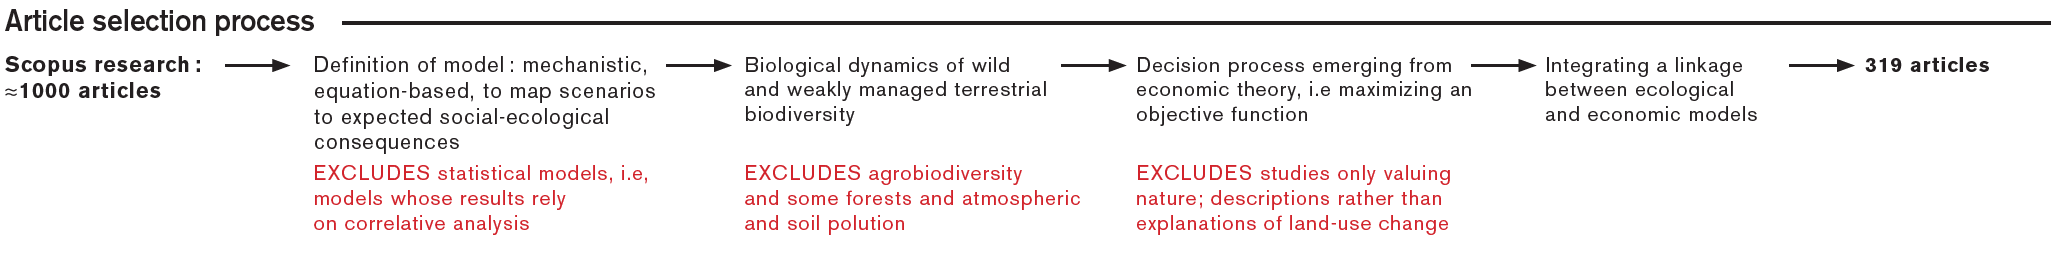
\includegraphics[width=\linewidth]{figures/review/selection_process.png}
    \caption{Article selection process for inclusion in the systematic review}
    \label{fig:selection_process}
\end{figure}


First, we need to precise the definition of \textit{model} we used for this review. Indeed the modeling literature usually mixes scenarios and models which are  both used to provide information to support policy and decision making. However they refer to two different modeling components:
scenarios describe plausible futures for drivers of change and options for altering the course of these drivers through policy and management interventions while models enable scenarios of change in drivers to be
translated into expected consequences for social-ecological systems \citep{IPBES2016}. Adopting a methodological perspective of the field instead of a public policy one, we will focus here on models only. Nevertheless, different types of models coexist in the literature. They can rely on quantitative relationships between the components of the social-ecological systems, or on qualitative relationships between them. While the first ones usually have mathematical foundations, the second ones are expert-based. In those models, the experience of experts and stakeholders, including local and indigenous knowledge holders, is used to describe relationships. In consistency with the bioeconomic models popularized by Clark about fisheries, we restrict our attention to quantitative models.
Eventually, the scientific literature distinguishes 2 types of quantitative models. On the one hand, the correlative models which rely on empirical data and estimate values for parameters through statistical relationships. In these models, processes are rather implicit. Second, the process-based models which describe explicitly-stated processes or mechanisms based on established scientific understanding. In these models, model parameters therefore have a clear and predefined interpretation. The scope of our review focuses on process-based bioeconomic models. This is of special interest since correlative modelling  is probably the best known to manage social-ecological systems, especially due to the popularity of correlative species distribution modelling \citep{Elith2009}. In such a context, we postulate that a specific focus on the alternative method might bring new insights about social-ecological system management.



Second, bioeconomics is a polysemous term which is used in different strands of literature: a first group is related to  N. Georgescu-Roegen and develops a thermodynamics understanding of social-ecological systems \citep{GeorgescuRoegen}; a second group, led by Clark on Gordon's and Schaeffer's foundations, develops mathematical models integrating ecological and economic processes  \citep{Clark630,Clark73, schaefer_some_1957}\footnote{See \cite{Parent_Mouysset_Missemer_Levrel_2024} for a history of the `standard' fishery model, notably the gradual inclusion of dynamics} ; finally a third group is related to biomimetism where technological innovations are inspired by living systems \citep{VANLANCKER201660}.
In this review, we focus  on the second group of literature, related to Clark's bioeconomic mathematic modeling.

To do so, we define bioeconomic models at the intersection of 3 conditions:
\begin{enumerate}
\item integrating an explicit biological dynamic 
\item integrating a decision process emerging from economic theory,
\item integrating a linkage between ecological and economic models.
\end{enumerate}

The first item characterizes the ecological dynamics of a renewable resource where the rates of regeneration and extraction are  commensurable.  Except for this condition, no specific requirement of the ecological process at play is needed. Different ecological processes such as population dynamics or niche distribution are thus eligible. 
By biological, we mean that the dynamics have to be related to living organisms. In other terms, the stake of the model has to be related to biotic elements. This condition aims at excluding pollution models or carbon and nitrogen models \citep{Nordhaus94,Lemoine2014}.
Eventually, by explicit we mean mathematically formalized. This condition is necessary to exclude exclusively declarative bioeconomic models (\textit{i.e} bioeconomic frameworks without any mathematical formulation). Indeed, the objective of this study is focused on changes in a specific method (\textit{i.e} the mathematical process-based bioeconomic model) rather than in a problem (\textit{i.e} the bioeconomic one). Because they adopt a different methodological framework, correlative or declarative bioeconomic studies need to be excluded from our corpus. 

The second item precises the economic side of bioeconomic models. 
By considering an economic decision process, we aim at excluding articles performing an economic valuation of biodiversity such as empirical studies giving the monetary values of species, like owls or bats \citep{MONTGOMERY1994,BeesCVM}. Although such studies are highly valuable to deal with the ecological crisis, they stem from a very different methodological tradition (choice experiments and monetary valuation). By explicitly requiring a decision process from economic theory, we ensure to avoid agro-ecological models. Indeed, many agro-ecological models address the question of sustainable management of terrestrial social-ecological systems and bring valuable knowledge to this question. However, they combine ecological dynamics with land-use change models without specifying the economic determinants of these land-use changes (some costs are sometimes associated with these land-use changes but without being driven by economic processes) \citep{SABATIER2010}. The methodological corpus we are interested in in this article is rooted in economic theory. Thus, we only consider economic decision models, in which agents allocate scarce resources to fulfill their objectives. Agents can, for example, maximize their utility or profit, or act as cost-minimizers to achieve specific goals. 

The third condition is that of an integrated ecological-economic system, \textit{i.e}, how the ecological and economic models are coupled. This bioeconomic linkage is not specified and can take different forms: for example, it can be mutual (by considering simultaneously the anthropogenic effects on ecosystems and the economic valuation of biodiversity in an economic problem) or unidirectional (one of the two effects mentioned above), and it can be done by prices or by physical variables. If the bioeconomic coupling is done by prices, economic value will be granted to the biodiversity elements to make them commensurable with other economic determinants. However, this monetary quantification has to be incorporated into a decision model (cf previous item).

Eventually, these bioeconomic modelling specifications have been applied to terrestrial social-ecological systems. Since many studies take place in an agricultural context, it is necessary to specify here the distinction between \textit{agro-biodiversity} and \textit{agricultural biodiversity}.\textit{ Agro-biodiversity} stands for species which are directly managed by farmers (for examples the crops species, the battle species etc) while \textit{agricultural biodiversity }stands for wild biodiversity living into agricultural habitats (such as birds, bats etc). Because the economic aspects of agro-biodiversity  have been broadly studied by agricultural economics, we focus here on wild terrestrial biodiversity. In this perspective, bioeconomic models applied to only managed forests, such as the seminal article of \cite{Faustmann}\footnote{Moreover, Faustmann's work focusing on tree values does not feature any biological dynamics.}, are excluded. Models with natural forest ingrowth are however in our scope. To finish, we formally exclude articles with marine case studies. For example, articles with both marine and terrestrial case studies have been excluded in this review. In doing so, we aim at providing a restricting view about terrestrial social-ecological system management. However the integration of such excluded articles appears as a natural perspective of future extensions of this work.

Based on these criteria, we individually screened all the papers selected in the first look to refine our database. Among 1000 articles identified after the first literature screening, we selected 319 articles developing bioeconomic models applied to terrestrial social-ecological systems.


\subsection{Analytical framework}

To analyze  mathematical tools such as bioeconomic models, we adopted here a methodological perspective. However as mentioned by Gibbard and Varian \citep{GibbardVarian} at an early stage, stories are an integral part of the model in economics. More precisely, the authors explain that a model is a \textit{story} with a \textit{specified structure}\footnote{"\textit{A model [...] is a story with a specified structure. The structure is given by the logical and mathematical form of a set of postulates, the assumptions of the model. The structure forms an uninterpreted system [...] Although the term ‘model’ is often applied to a structure alone, we shall use it in another sense. In economists’ use of models, there is always an element of interpretation: the models always tells a story.}" \citep{GibbardVarian}, p.666)}. In that perspective, methodological specifications are not sufficient to  characterize the model since the questions the authors want to explore and the stories they can tell with it are at the core of the model identity. Such narrative elements are more than chronicles, they are essential to connect economic modeling research with the specifics of the world \citep{Morgan}. Without these narrative elements, it is impossible to apply model-structures directly onto the facts of the economic world. Since we are interested in models that are motivated by concrete stakes such as resource management, the biodiversity crisis and sustainable development, exploring narratives associated with the methodological specifications of the mathematical model is crucial to characterize the outline of such a bioeconomic modeling. 

In this context, we developed an analytical framework based on two dimensions: the first one is based on a set of methodological criteria related to mathematical equations, while the second one is related to the narratives associated with the mathematical tool. Based on the combination of these two dimensions, we aim at providing an overall cartography of bioeconomic modeling as a tool to investigate the management of terrestrial biodiversity.

\section{Cartography method}

For our methodological analysis, we first investigated a set of 18 criteria related to the ecological model, the bioeconomic linkage, and the economic model. 

\subsection{Ecological criteria}

The ecological criteria aim at precising how biodiversity is captured by the ecological model. To do so, we mobilize 8 criteria split into 2 groups. The first group of criteria helps to understand the paradigm of biodiversity while the second group is  related to the technical specifications  of the ecological model.

Within the first group, the first criterion is related to the  measure of biodiversity. Indeed, biodiversity can either be modeled \textit{per se} (for example based on population dynamics models) or be deducted from a proxy (typically, the habitat suitable for biodiversity or economic activity). The second criterion precises the proxy measure: this proxy can be habitat, economic activity, a conservation budget, or not be specified. 
The third criterion precises the ecological state variable in the ecological model. More precisely, the biodiversity variable can be related to the individuals (such as in population or metapopulation models), the species (when focusing on species richness), or the community, when both species abundance and richness are taken into account. 
The fourth criterion focuses on the type of biological diversity, \textit{i.e.} we distinguish functional and genetic diversity definitions. 
Finally, the fifth criterion characterizes the biodiversity level at which the model intends to contribute. Some articles are focused on a single species (for example, articles based on a population model developed for one species) while some others adopt a community perspective by integrating a pool of species. In some cases, when species interact, models display two species. However, many of the articles we reviewed did not focus on species interactions and therefore encompassed a larger number of species. This community perspective can be either explicit, as in articles modeling populations of different species, or implicit, in studies using a habitat proxy as a biodiversity measure and informing about the community living in this habitat. It is interesting to note that there is no systematic implications between habitat, proxy-based models and community level contribution since the habitat might be related to one single species. 

Besides this first group of criteria for the characterization of biodiversity, we mobilize a second group of criteria related to the ecological technical specifications. The first criterion is related to the category of biological dynamics: we distinguish population dynamics models (such as in the seminal model developed by Clark, or articles implementing age-structured modeling) and other ecological dynamics. These other dynamics can be for example either a niche distribution model or Brownian motion models. The second criterion characterizes the spatial dimension of the ecological process. Spatial considerations can be explicit when the ecological process implies spatial exchanges (typically a meta-population  model) or implicit, when the ecological process at play takes place in a heterogeneous context (for example when heterogeneous patches are taken into consideration for an aggregated analysis without any exchange between the patches). Eventually, the spatial dimension can be absent. Then the third criterion is related to the integration of stochasticity in the ecological modeling. Stochastic components may include dispersal probabilities of species across land patches as well as probabilities of species extinction.

Table \ref{tab:database_methodo} sums up the ecological criteria with their related items.

\subsection{Bioeconomic linkage criteria}

 Bioeconomic linkage criteria characterize how biodiversity is taken into account in the economic model and the economic decision. To do so, we mobilize 3 criteria. 
 The first criterion indicates whether the biological element has been monetarized or not. In order to make biodiversity commensurable with other economic variables in the decision problem, some articles rely on an economic valuation of biodiversity (in other words, biodiversity is expressed in monetary units, such as dollars). A monetary bioeconomic linkage occurs in two situations: either if the study is directly driven in monetary terms (for example when biodiversity is measured through a proxy in economic units) or if the ecological model is developed in non-monetary terms (with a biodiversity measure \textit{per se} or based on a habitat-based proxy) but the biodiversity is monetarized thanks to a monetarization method to be integrated into the economic decision.

The second criteria precises how the bioeconomic problem is raised. We distinguish two problems: the cost-benefit problem and the cost-effective problem. Cost-benefit analysis integrates costs and benefits related to classical economic factors and ecological factors, then selects the decision which maximizes the overall utility. Due to criticism on monetarization methods \citep{Diamond94}, some authors favor cost-effectiveness analysis which separates classical economic factors and the ecological ones. The economic decision is thus taken according to a maximization under constraints. Typically, the optimal decision maximizes the profit or the utility under an ecological constraint.  By isolating ecological and economic objectives, this cost-effectiveness method aims at limiting the substitutability between natural and non-natural capital. 
Interestingly some studies consider the ecological value in economic terms (for example when biodiversity is measured through an economic proxy) but keep separated the benefits or costs emerging from the ecosystem  and the ones emerging from classical economic factors. In other terms, an economic value for biodiversity does not necessarily imply a cost-benefit problem. It is the reason why it is informative to keep in our review the two criteria, relative to biodiversity monetarization and the bioeconomic problem respectively.

The third criterion captures the position of the biodiversity stake in the bioeconomic model. The biodiversity stake can be within the objective of the maximization such as in cost-benefit problems but also in a cost-effectiveness problem which
maximizes the ecological output while satisfying a cost constraint. Then, the biodiversity stake can be a constraint (in a cost-effectiveness problem which maximizes profit under ecological constraint for example). Eventually, other stakes occur either when the biodiversity stake emerges in both the maximization and constraint or when the biodiversity stake is an output. The simultaneous consideration is possible when are considered different taxonomic groups (one being in constraint while the other is included in the maximization) or when non-human well-being is taken into consideration in the objective function while biological dynamics constitute mechanistic constraints. The biodiversity stake can be assessed as an output computed after the economic decision. 

Table \ref{tab:database_methodo} sums up the bioeconomic linkage criteria with their related items.

\subsection{Economic criteria}

Economic criteria specify the economic side of bioeconomic models. More precisely, we explore a set of criteria related to the technical economic specifications. They are related to dynamics \footnote{Indeed whereas our definition of bioeconomic models requires a condition of dynamics in the ecological model (see section \ref{sec:art_selec}), we do not impose any dynamics specifications on the economic side to be included in the database.} and spatial dimensions, and to uncertainty. 
Bioeconomic models are economically either static or dynamic. Similarly to ecological technical specifications, we explore the spatial and uncertain dimensions. Economic spatiality can be investigated explicitly through a spatial process such as trade between regions or implicitly by spatial heterogeneity of economic variables, or eventually absent of  bioeconomic models. Eventually, economic models can be either deterministic or stochastic if an economic variable is primarily subject to a source of uncertainty. 

To finish, we explore four last criteria regarding the general characteristics of bioeconomic models. The first one is related to the solving method used to explore the bioeconomic question.
We distinguish 3 forms of solving method in the articles of our corpus: closed form resolution, numerical resolution and the combination of both. The second criterion informs whether the study is empirical or theoretical or whether its combines empirical and theoretical perspectives. 
Additionally, we explore how the model is used to highlight the economic question. If the solution emerging from the bioeconomic model characterizes a judgement on the best behavioral options or policy instruments, the model use is normative. On the other hand, if a paper investigates some behaviors of the system without any recommendation, the model use is descriptive.
Eventually, we characterize whether the model is framed in terms of general equilibrium or partial equilibrium. 

Table \ref{tab:database_methodo} sums up the economic criteria with their related items.

\subsection{Methodology-based cartography}

These methodological criteria have been analysed through a Multiple Correspondence Analysis (MCA). MCA allows to uncover the underlying structure of categorical data by performing a recomposition of the data into a two-dimensional space formed by orthogonal vectors which maximize the variance (inertia) explained by the data (see \cite{Benzecri} for seminal works and \cite{LeRoux_Rouanet} for a modern presentation).

As MCA can be sensitive to unbalanced variables (\textit{i.e.} variables whose distribution are highly skewed towards one value), we performed a sensitivity analysis to select the optimal combination of variables to use in the MCA, based on the explained variance. To do so, we performed an MCA analysis with all the possible combinations of our sample.
The graph \ref{fig:nb-crit-methodo} in appendix \ref{appendix:graph} exhibits the explained variance as a function of the number of criteria. Among the 18 methodological criteria, we selected the set of 14 methodological criteria (see tab. \ref{tab:database_methodo}) which keeps a large set of criteria  while reaching 31\% of the explained variance. The rationale for variable selection was to avoid redundancies as well as excluding variables that are too skewed and would impair MCA analysis. 
%

Based on these selected criteria, we performed a classification with a K-modes algorithm (\cite{Huang1998}). The K-modes algorithm generalizes the K-means method\footnote{ The K-means algorithm \citep{mcqueen1967,Lloyd1982} is a standard classification algorithm in Natural Language Processing. Documents are mapped to a vector space featuring as many dimensions as there are distinct words in the document, and are thus coded in a binary fashion. The algorithm picks random initial centroids, computes the Euclidean distance to other observations, which are assigned to the closest clusters. Centroids are thus actualized, and the procedure is repeated. If no observations changes cluster upon a new iteration, it converges.} to categorical data, and uses a dissimilarity measure to assign observations to clusters. One of the inconvenients of K-modes algorithms is the need to specify to number of clusters. Therefore, the number of groups used in the classification was determined using a cost function, namely the sum of the within variance of each clusters. We used the so-called 'elbow-method' (\cite{Ketchen1998}), stating that the optimal number of clusters is located at an elbow of the curve relating the sum of the within cluster variances and the number of clusters. Indeed, after this point, the reduction in the sum of the within cluster variances becomes less important, suggesting additional clusters do not significantly improve results. Figure \ref{fig:cost-function} in appendix \ref{appendix:graph} depicts this cost function. For the following analysis, we will consider the optimal cluster of 4. However since 9 clusters might also be considered as optimal clustering, we also present an MCA classification with 9 clusters as robustness test (see figure \ref{fig:MCA-9groups} in appendix \ref{appendix:graph}). 


\subsection{Narrative-based analysis}

In order to perform a narrative analysis, we used the titles, keywords and abstracts of the papers in our database.
Then we pre-processed the data by removing stopwords and grouped similar words together (for example, \textit{farming}, \textit{farmers} and \textit{farms} were all grouped under \textit{farm} with this procedure). Moreover, because our analysis relies on single words, typical nominal groups were recoded (for example, \textit{endangered species} was recoded into \textit{endangeredspecies})\footnote{The following expressions were recoded and grouped together : endangered species, bio-economic, invasive species, ecosystem service, optimal-control, dynamic-programming, integer-programming, cost-effective, cost-benefit, reserve-design, optimal-management, land use, property rights, conservation-planning} .
%
For our analysis, we kept words which occurred at least 5 times in our database\footnote{These 5 occurences can come from a single article or at most 5 articles.}. Since we have 319 articles, we thus kept a significant portion of the words database, which displays the most information. More precisely, a total of 1202 words out of 4355 relevant words (27.6\%) were kept, accounting for 81\% of word occurrences.

Eventually, we classified words according to semantic fields. Based on the 1202 words words kept for the analysis, we designed 8 lexical groups, pertaining to two habitats (agricultural and forest), two species status (invasive species and endangered species), two management semantic fields (policy and risk) and two human-nature paradigms (conservation and harvesting). The list of words in each semantic field is depicted in appendix \ref{appendix:lexical_groups}. 
In order to characterize the narratives underlying the different groups resulting from the methodology-based classification, we investigated the bias of each semantic fields into them. More precisely, for each methodology-based group, we assess the ratio between the frequency of the semantic fields and the number of papers included in this group. This ratio avoids size effects between groups.





\section{Database overview}

\subsection{Temporal and geographical distributions}

Figure \ref{fig:distrib} presents the distribution of the articles in the database. Most articles range from the 90's, testifying the recentness of the use of such methodology for terrestrial social-ecological systems.  
Except some early-bird articles published in the 70's related to the management of agricultural pests and pesticides use \citep{Hueth1974,Feder1975}, the distribution of the articles follows a Gaussian function with a 20-years spike between 1995 and 2015. This indicates that the use of such bioeconomic models to investigate the sustainable management of terrestrial social-ecological systems has decreased recently. This  decline is of special interest  as  the question of sustainably managing terrestrial social-ecological system is far from solved. This situation is quite unusual for a methodology associated with such a burning issue which calls for a strong research effort and generates a huge amount of literature.

\begin{figure}
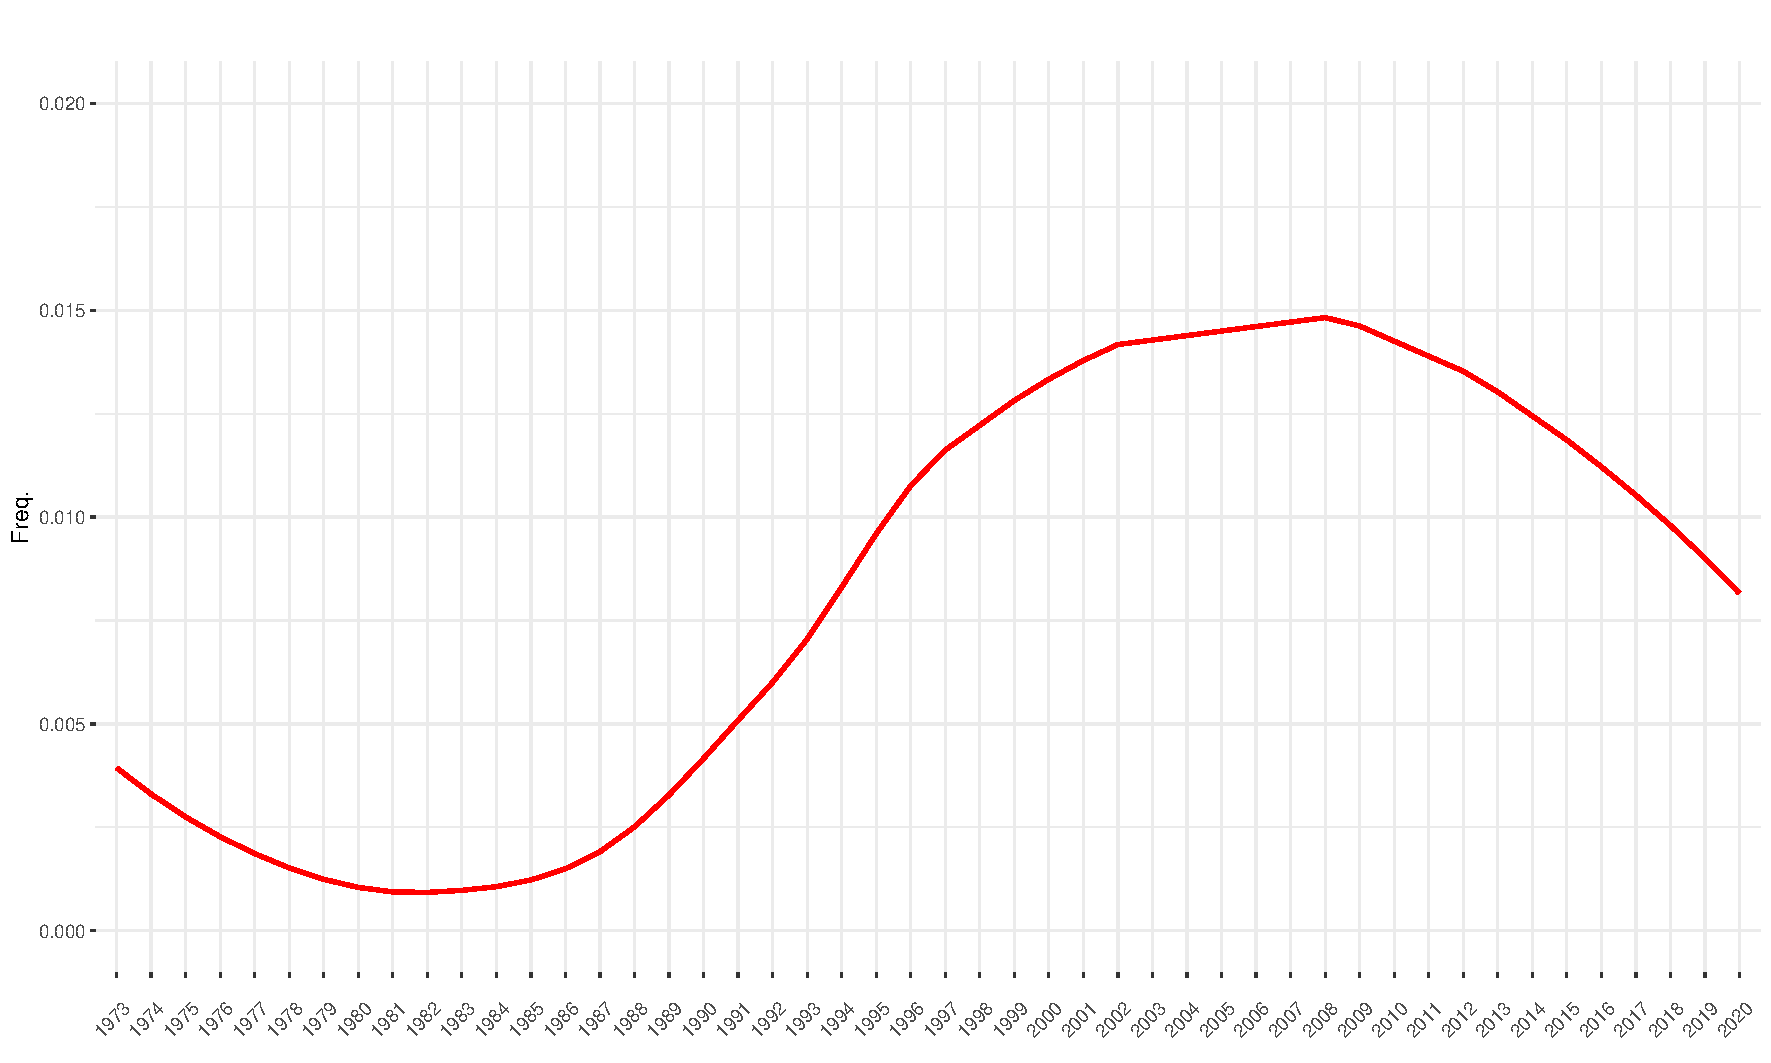
\includegraphics[width=.8\textwidth]{figures/review/temporal_distribution_full.pdf}
\caption{\label{fig:distrib} Temporal distribution of articles in the database.}
\end{figure}

To complete this temporal distribution, we investigate the geographical origins of the authorship of the 319 articles (fig. \ref{fig:distrib-geo}). 
We observe that our database in majority emerges from North American and European research even if the part from Oceania is not negligible. Eventually a small part comes from Asia and Africa. This relative dominance of North American research could be explained by the original diffusion of Schaeffer's (American) and Clark's (Canadian) seminal models. From a more naturalist stand, the magnitude of the resources and the early conservation movement in North America could have paved the way for this trend.

\begin{figure}[h]
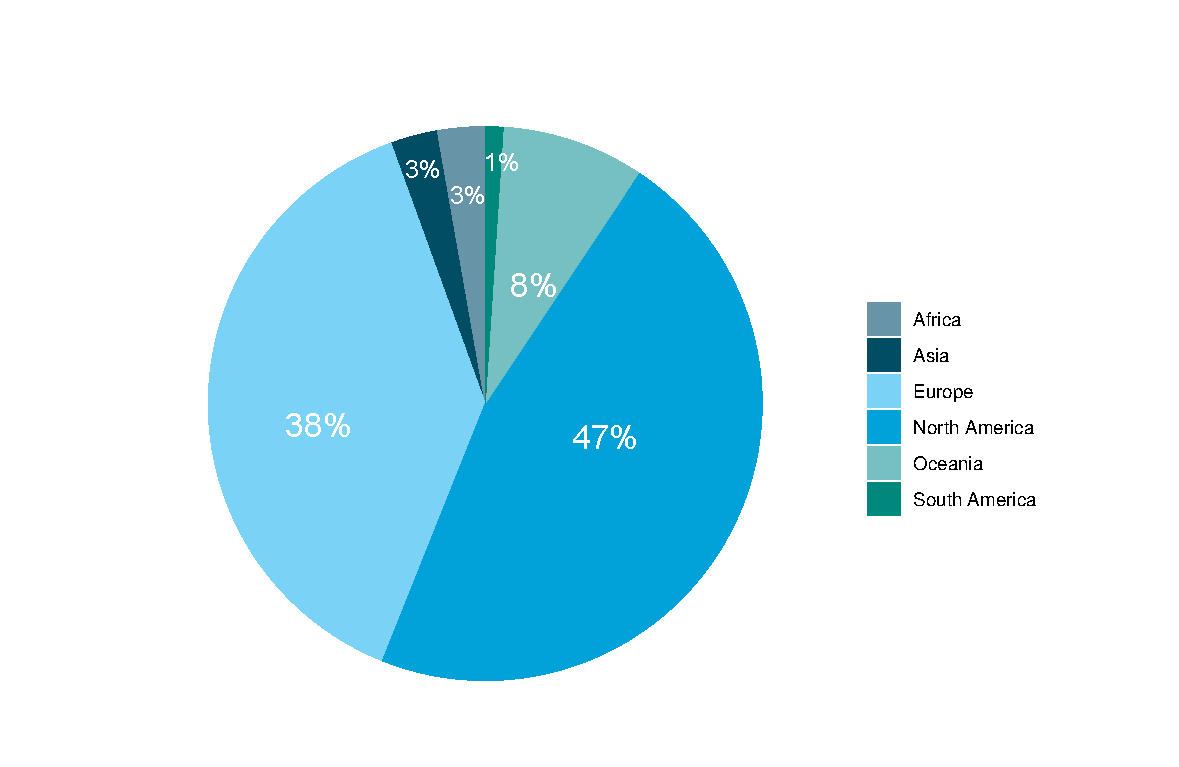
\includegraphics[width=.8\textwidth]{figures/review/pie_geographic_whole_base_method2.pdf}
\caption{\label{fig:distrib-geo} Geographical distribution of articles in the database.}
\end{figure}

However with a higher pressure on land use and land use change in Europe than in the USA, European researchers look also very active to face the urgent and concrete stake  of managing terrestrial ecosystems while reconciling socioeconomic goals and ecological requirements.
%\clearpage
%
\subsection{Journal and discipline distributions}
The articles emerge from 97 journals which are related to different disciplines such as applied mathematics, economics, ecology and sustainability sciences (see tab. \ref{tab:journal_disci}). Based on the journal affectation, table \ref{tab:journal_field} sums up the frequencies of these 3 disciplines among our corpus of 319 articles.

\begin{table}[!htbp] \centering 
  \caption{Distribution of journal across fields} 
  \label{tab:journal_field} 
\begin{tabular}{@{\extracolsep{5pt}} ccc} 
\\[-1.8ex]\hline 
\hline \\[-1.8ex] 
Field & Count & Percentage \\ 
\hline \\[-1.8ex] 
Economics & $190$ & $60\%$ \\ 
Ecology & $83$ & $26\%$ \\ 
Sustainability science & $34$ & $10\%$ \\ 
Applied Mathematics & $12$ & $4\%$ \\ 
\hline \\[-1.8ex] 
\end{tabular} 
\end{table} 

We observe that most of the articles have been published in journals related to economics (60\%) confirming the anchorage of bioeconomic modeling as an economic approach. Among the journals, one of them captures a substantial part of the papers: 44 papers (\textit{ie} 14\% of the overall database and 23\% of the papers published in economic journals) are indeed published in \textit{Ecological Economics}. This dominance was expected since the methodology brought by bioeconomic modeling fits perfectly with the scope of the journal. Indeed, this journal focuses on the articulation of ecological and economic issues in the perspective of sustainable development\footnote{The scope of \textit{Ecological Economics} mentions that "\textit{The journal is concerned with extending and integrating the understanding of the interfaces and interplay between "nature's household" (ecosystems) and "humanity's household" (the economy). Ecological economics is an interdisciplinary field defined by a set of concrete problems or challenges related to governing economic activity in a way that promotes human well-being, sustainability, and justice}."}. Beside this journal, bioeconomic models contribute to  classical resource management questions (with environmental and energy journals such as\textit{ Environmental and Resource Economics}, \textit{Journal of Environmental Economics and Management}), applied questions and notably agricultural economic journals (such as in the \textit{American Journal of Agricultural Economics} or the \textit{Agricultural Economics}), theoretical economic questions (with classical theoretical journals such as \textit{Econometrica, American Economic Review}).


The  proportion of articles published in non-economic journals (40\%) testifies an interest for bioeconomic models beyond its economic expected arena.  
The non-negligible part of articles published in Ecology journals (such as \textit{Ecological Modeling} \textit{Conservation Biology}, \textit{Ecology Letters} or \textit{Journal of Theoretical Biology}), sustainability sciences journals (such as \textit{Natural Resource Modeling}, \textit{Agricultural Systems} or \textit{Environmental Modeling and Software}) and applied mathematics (\textit{Journal of Mathematical Analysis and Applications} and \textit{Journal of Mathematical Biology} for example) emphasizes an acceptance of bioeconomic models outside the field of economics. And more specifically, it confirms a certain legitimacy of bioeconomic models regarding ecological theory and knowledge. In this perspective, bioeconomic modeling embraces a genuine interdisciplinary aspiration.



\section{Database cartography}

\subsection{Methodology-based classification}

Figure \ref{fig:MCA}  presents the results of the Multiple Correspondence Analysis (MCA) running on 14 methodological criteria. It also displays the classification of the articles resulting from our K-modes algorithm into 4 groups : group 1, in green, with 47 articles; group 2, in purple, with 48 articles; group 3, in yellow, with 162 articles; group 4, in black, with 62 articles.

% (48 papers -resp. 47, 162, 62 papers- are in the group 1 -resp. group 2,3,4). 
%
We observe on figure \ref{fig:MCA} that the MCA is well structured on both sides of the \textit{y}-axis with groups 1 and 2 on the right side, and groups 3 and 4 on the left side. The \textit{x}-axis offers a split between groups 1 and 2 while it does not strongly play on the groups 3 and 4 even if the main part of group 3 tends to be below the \textit{x}-axis while the main part of group 4 tends to be above. Figure \ref{fig:MCA-9groups} in appendix \ref{appendix:graph} exhibits the MCA based on 9 groups. While being more fragmented, the cartography exhibits a similar structure to the 4 groups classification. 
\\
\hspace*{1.5em} The interpretation of the 4 groups comes with figure \ref{fig:MCA-motsclefs} which depicts the distribution of the items of the selected 14 methodological criteria. The colors stand for the contribution of the items to the structuration of the axes. We observe that the \textit{x}-axis is strongly driven by the criteria related to the bioeconomic problem e.g. biodiversity monetarization, data anchorage, solving method and spatiality. More precisely the left side is characterized by a cost-benefit problem where biodiversity is monetized. The problems are theoretical and solved with closed-form solutions. Eventually, the problems do not integrate spatiality. On the contrary, the right side is characterized by the cost-effective problem where biodiversity is not monetized. The problems are mainly empirical and solved with numerical tools, and take into account spatiality. The \textit{y}-axis is mainly driven by the integration of spatiality in the economic model and the framing of the economic problem as a general equilibrium. 
\\
\hspace*{1.5em} Combining figures \ref{fig:MCA}  and \ref{fig:MCA-motsclefs}, we understand that the MCA classifies the articles in our database in a first group (in green) specified by a cost-effective problem, an absence of biodiversity monetarization, empirical and theoretical studies and stochasticities being present both in ecological and economic models ;  a second group (in purple in figure \ref{fig:MCA}) specified by a cost-effective problem, an absence of biodiversity monetarization, empirical studies and spatiality being explicit on the economic side and implicit on the ecological side ; a third group (in yellow in figure \ref{fig:MCA}) specified by a cost-benefit analysis, biodiversity monetarization, numerical and theoretical solving and the absence of spatiality ; a fourth group (in black in figure \ref{fig:MCA}) specified by a cost-benefit analysis, biodiversity monetarization, theoretical solving and explicit spatiality.


\begin{figure}[H]
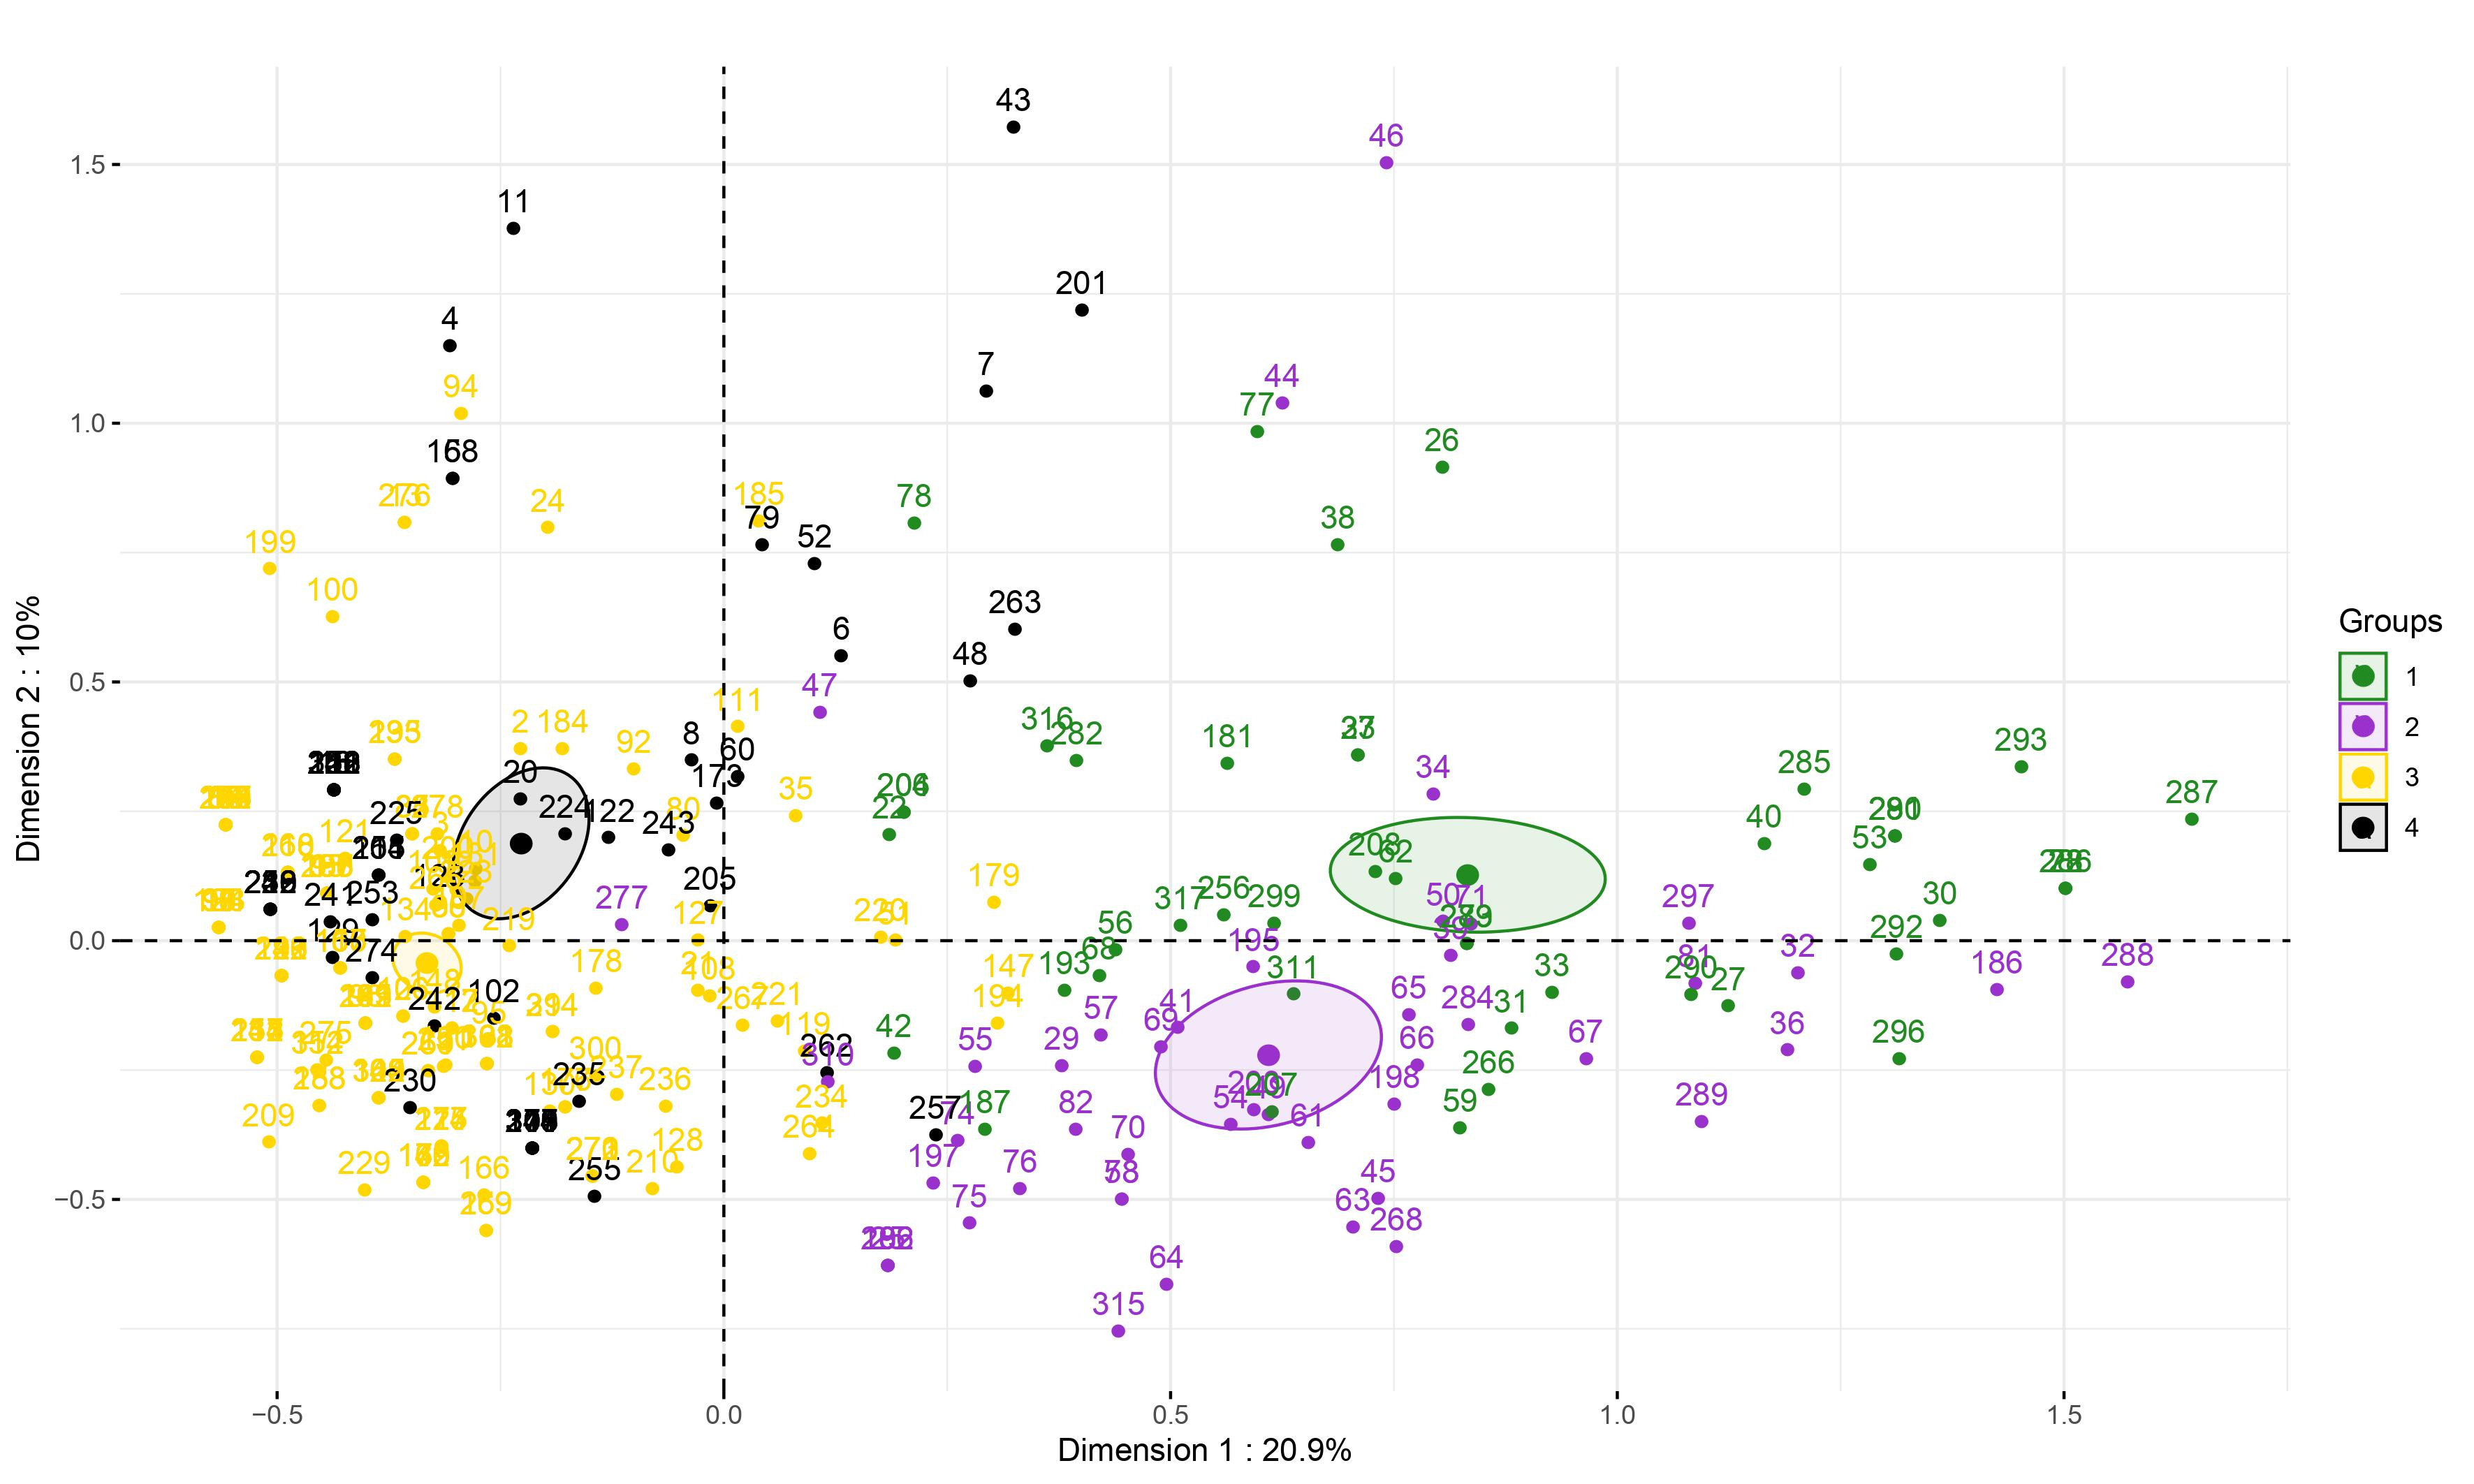
\includegraphics[width=.9\textwidth]{figures/review/mca_ind_automated_kmodes_rev.png}
\caption{\label{fig:MCA} Multiple Correspondence Analysis (MCA) running on 12 methodological criteria and 4 clusters (K-modes)}
\end{figure}
\begin{figure}[H]
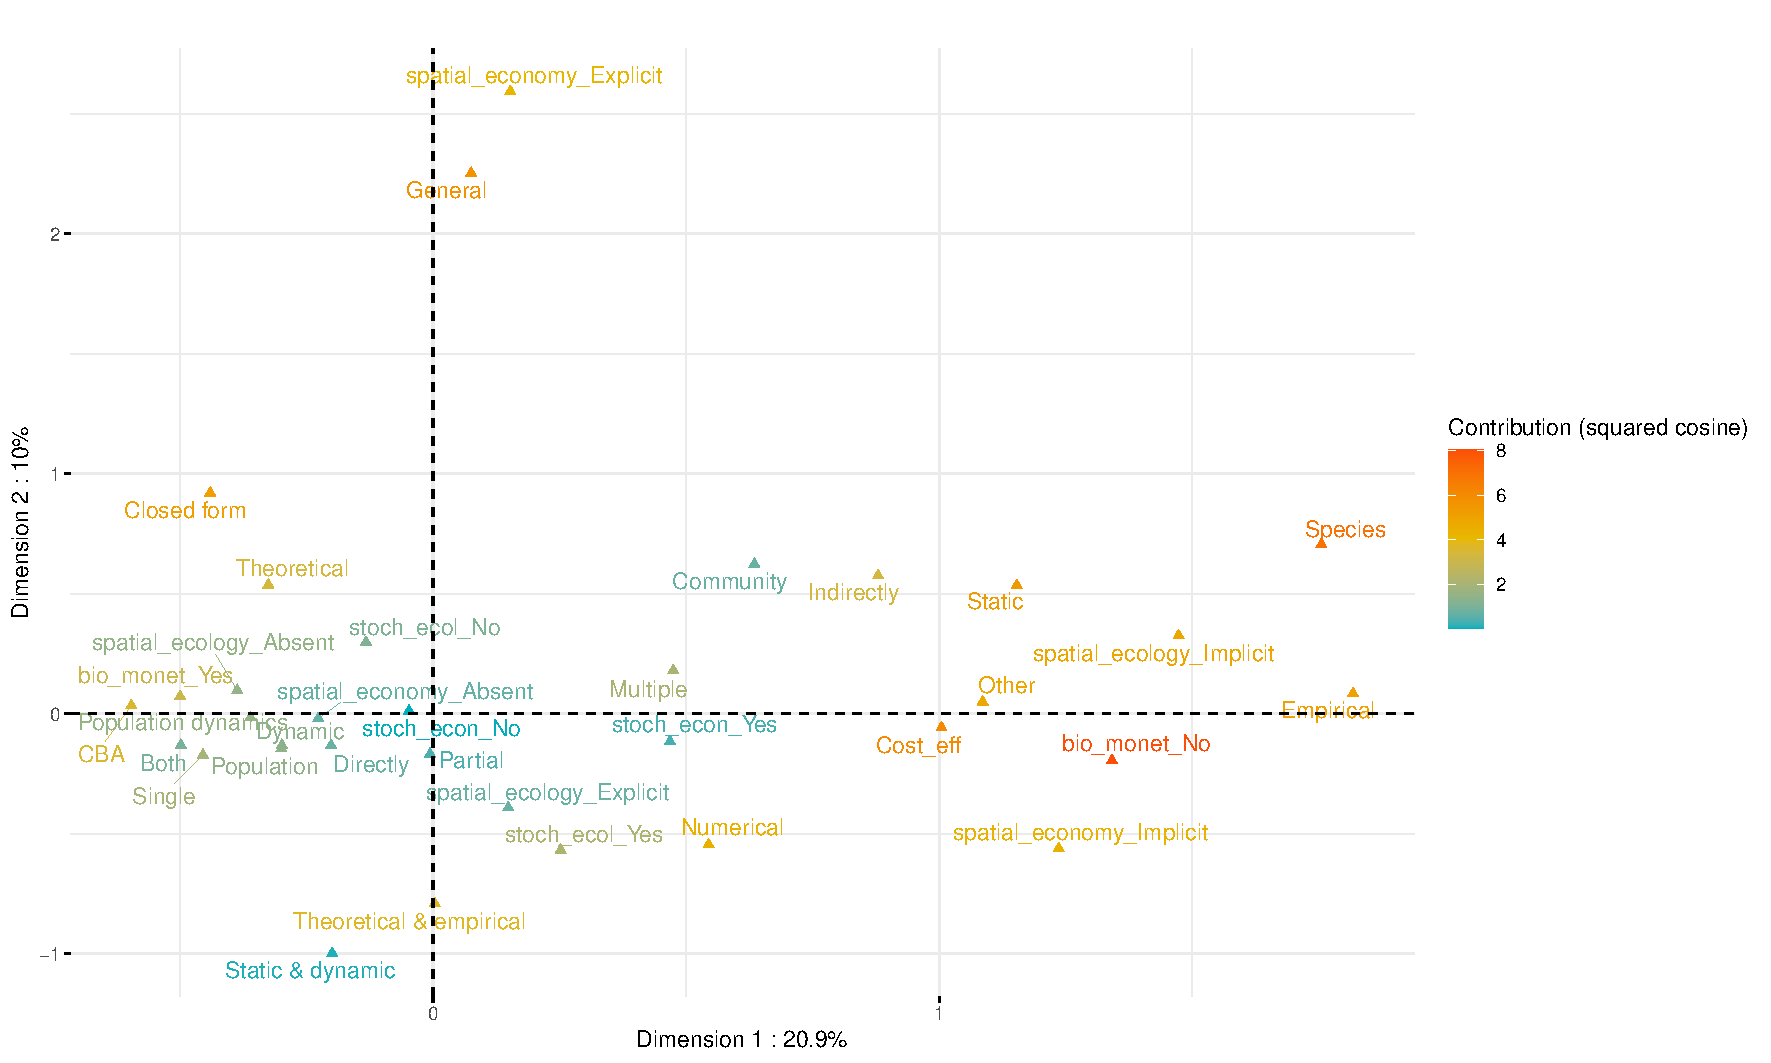
\includegraphics[width=.9\textwidth]{figures/review/mca_variables_automated.pdf}
\caption{\label{fig:MCA-motsclefs} Distribution of the values of 14 methodological criteria among the MCA axes.}
\end{figure}

\subsection{Narrative-based specifications}

In order to interpret the narratives of the 4 methodology-based groups, we depicted on figures \ref{fig:words-profile-1} and \ref{fig:words-profile-2} the distribution profiles of the 50 most frequent words for each group. 

First of all, we observe that for all profiles the most common words are those which are in common with the 4 groups.  We identified the following keywords: (i) economic, cost, (ii) management, policy, strategy, conservation (iii) biodiversity, resource, species, population, ecological, biological, (iv) model, optimal, dynamic, (v) land use, forest, habitat. This observation indicates that the 4 methodology-based groups are driven by a common narrative which regards an economic problem of management of biodiversity and natural resource and land use change based on models, mostly relying on optimal control theory. This result confirms the consistency of our database regarding the  research question investigated in the selected papers within the database.

Since the specific words are too disparate to be easily understandable, we completed these profiles by a semantic fields analysis in order to characterize the 4 methodology-based groups. The figure \ref{fig:semantic-fields} depicts the frequency of the different semantic fields in each group\footnote{see appendix \ref{appendix:lexical_groups} for the listing of words within each semantic field}. We observe that groups 1 and 2 are related to conservation issues. Among conservation-related articles, the ones with specific applications into agricultural landscapes, especially related to public policy issues, are preferentially located in  group 2. On the opposite, groups 3 and 4 are related to harvesting issues. A specific focus on endangered and invasive species characterizes  group 3. Eventually, group 4 looks dedicated to the risk problematic with forestry applications. 

\begin{figure}[h]
\centering
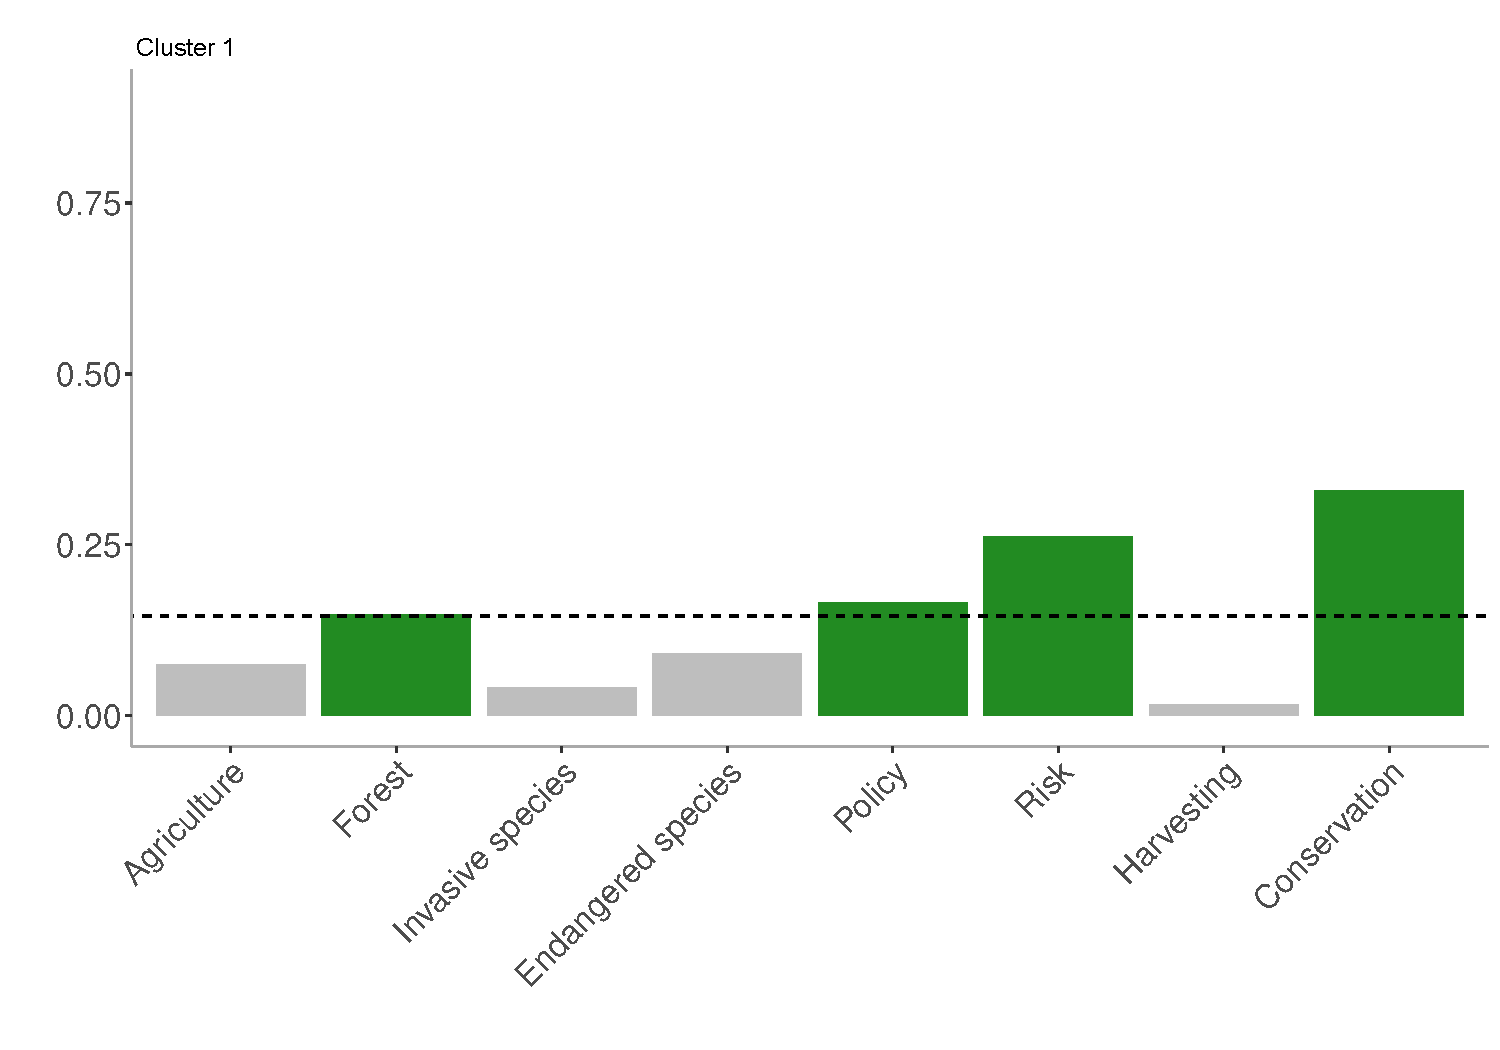
\includegraphics[width = .45\textwidth]{figures/review/lexical_profile_cluster_kmodes_bg2.pdf}
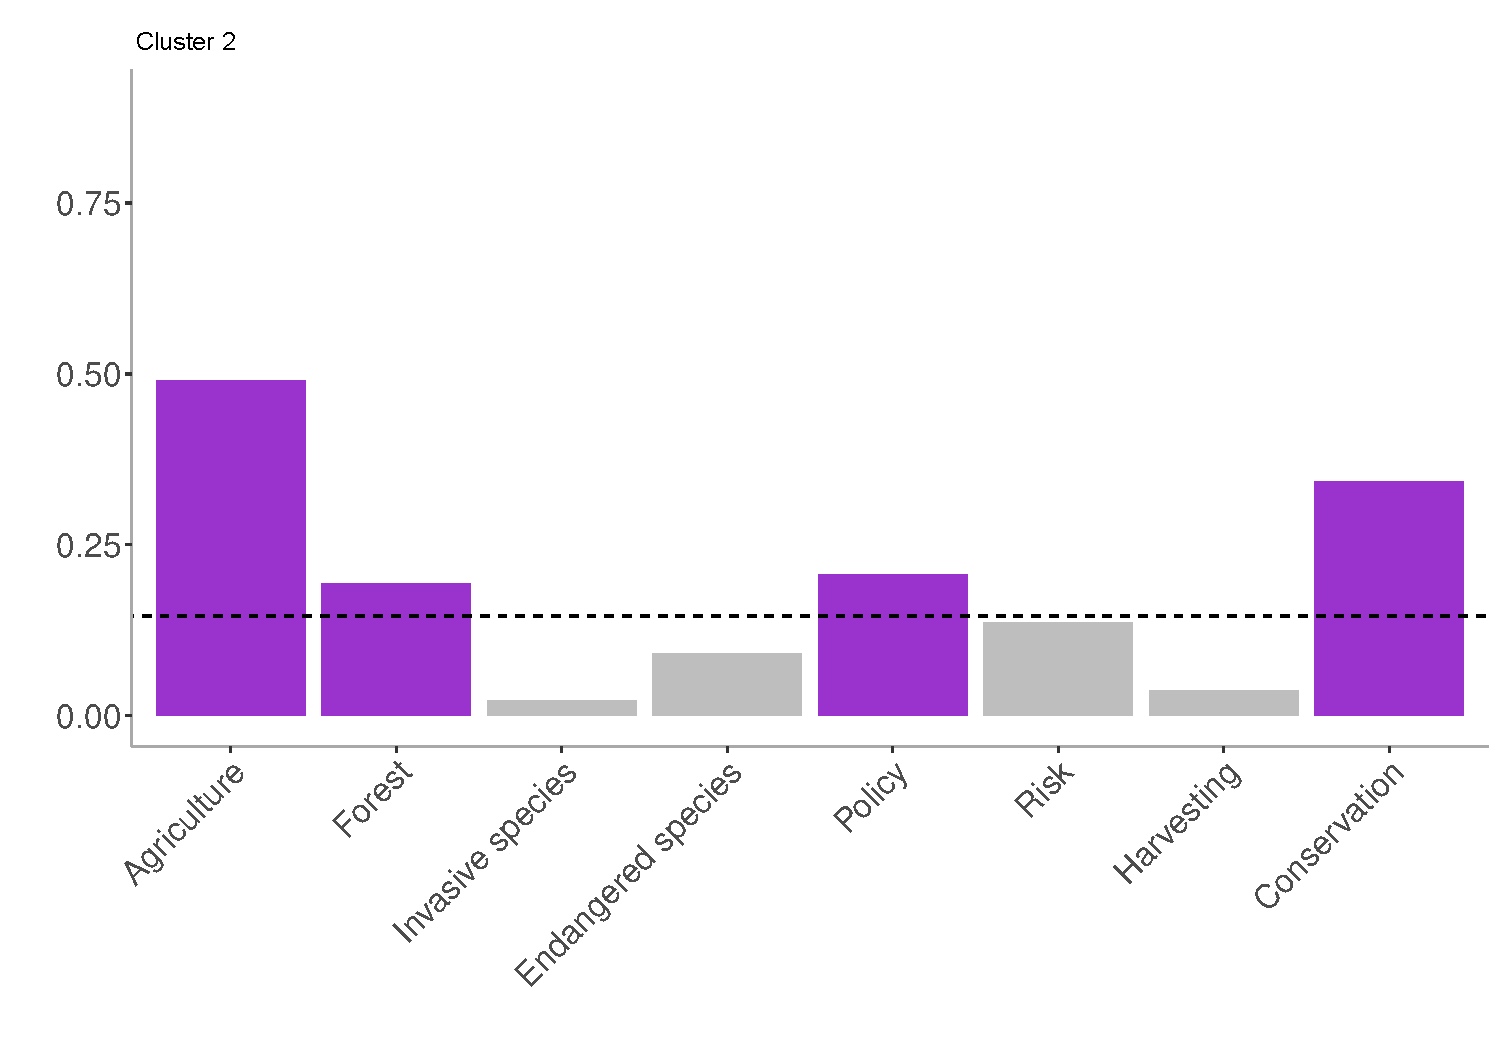
\includegraphics[width = .45\textwidth]{figures/review/lexical_profile_cluster_kmodes_bg1.pdf}\\
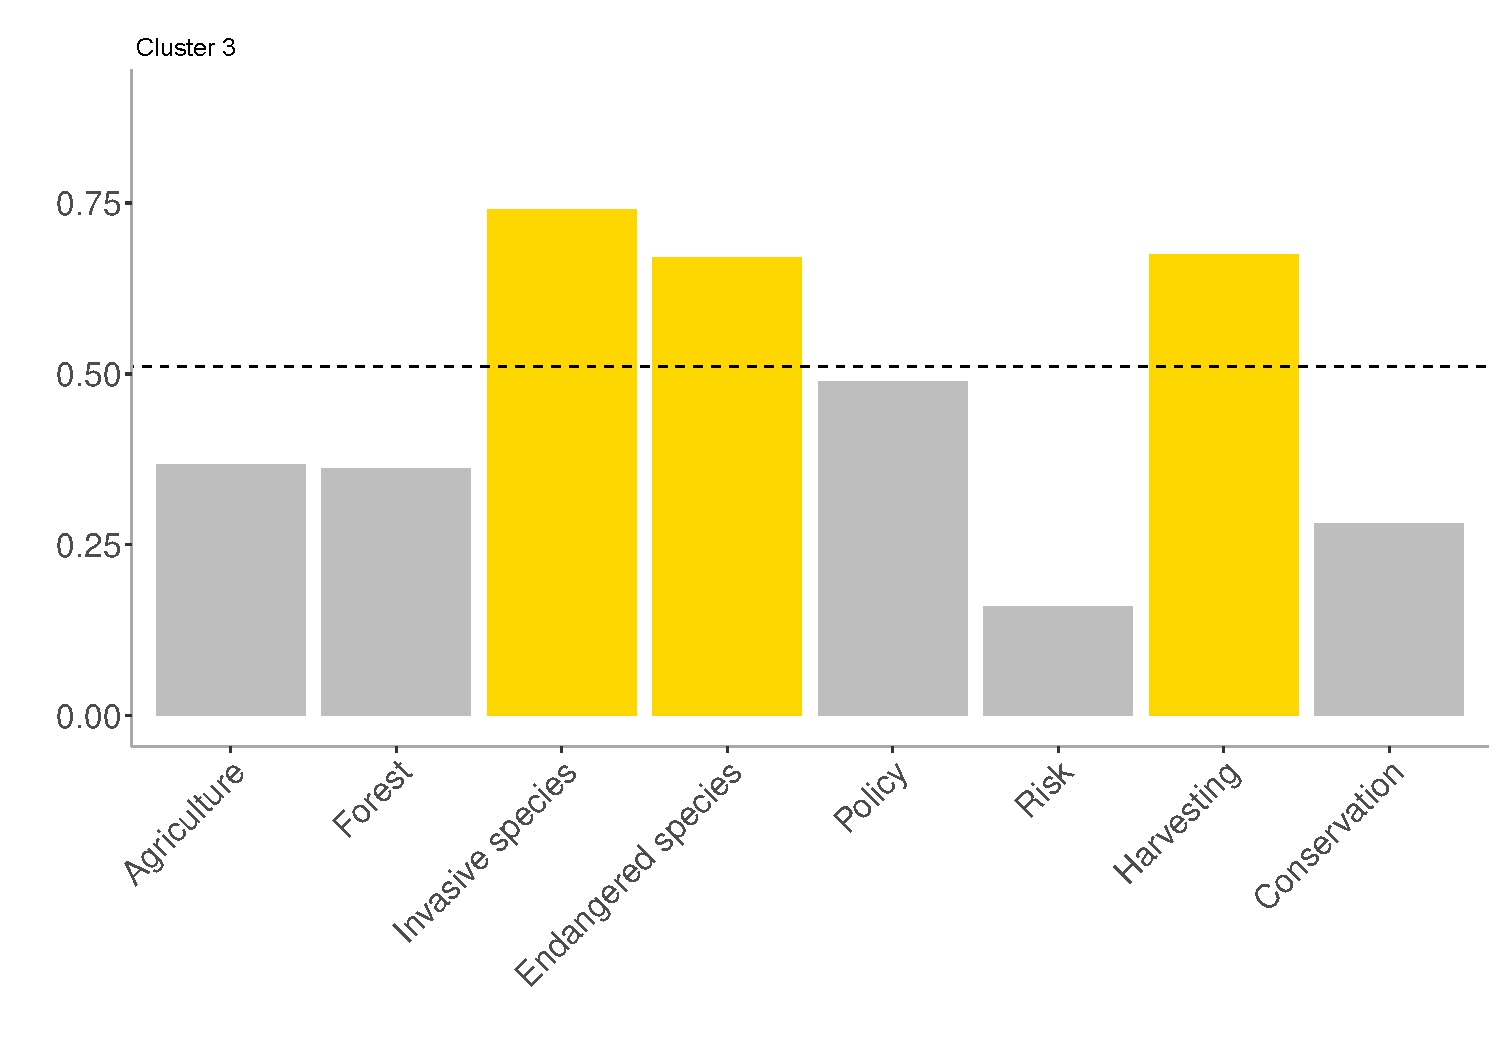
\includegraphics[width = .45\textwidth]{figures/review/lexical_profile_cluster_kmodes_bg3.pdf}
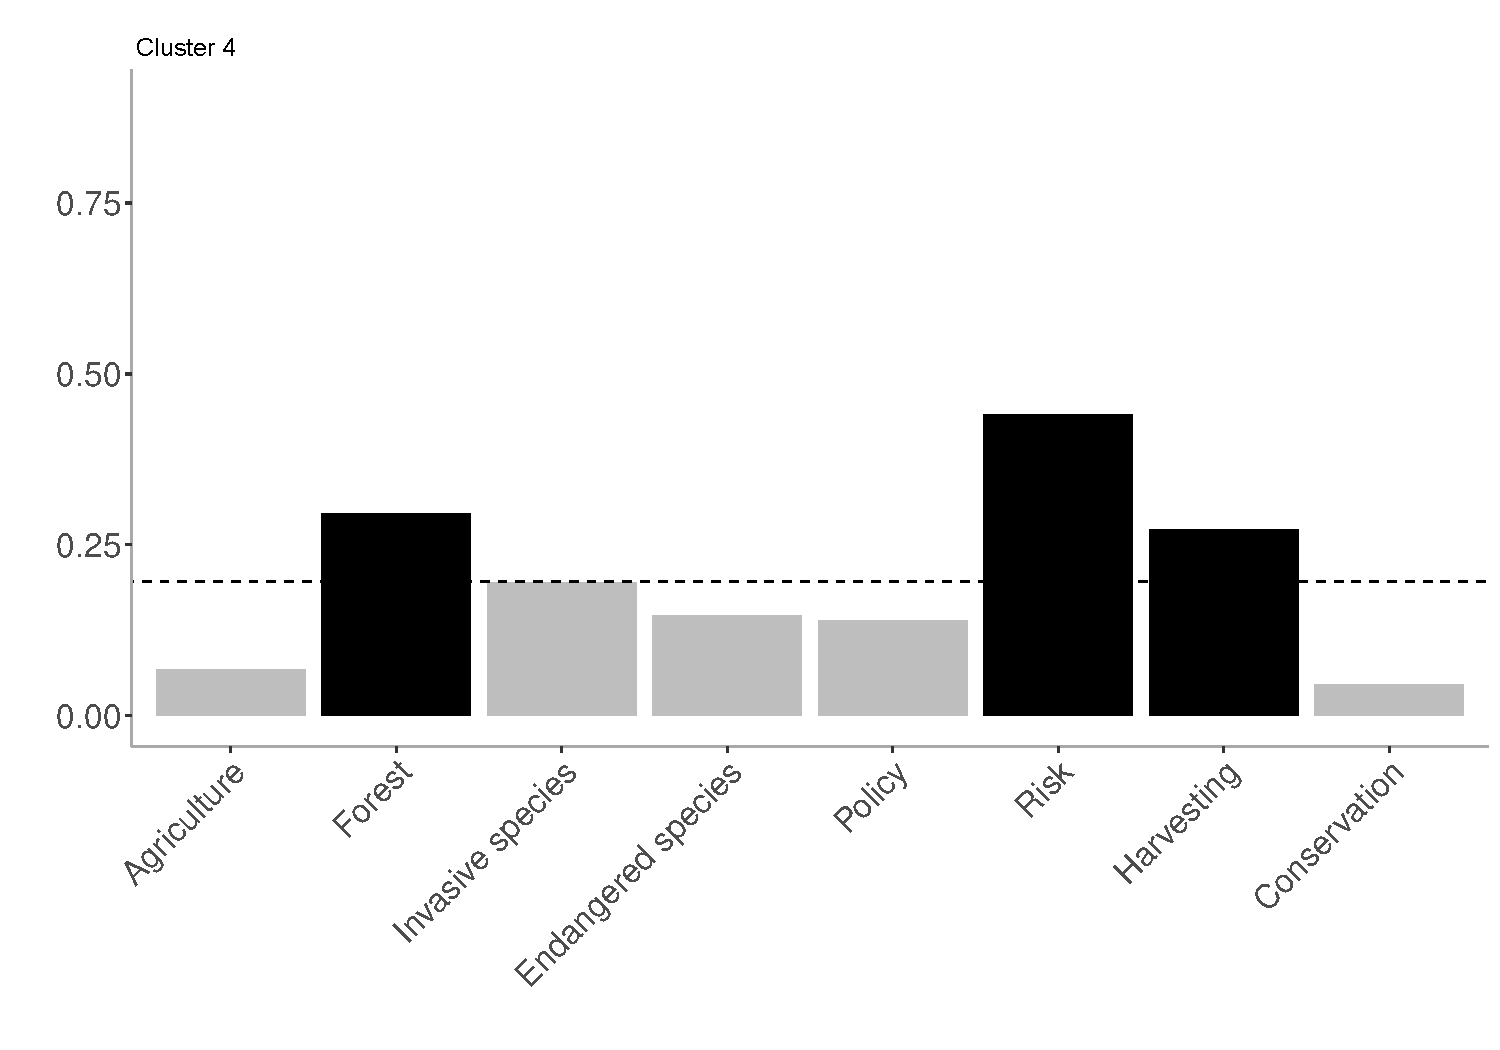
\includegraphics[width = .45\textwidth]{figures/review/lexical_profile_cluster_kmodes_bg4.pdf}
\caption{\label{fig:semantic-fields} Frequency of the different semantic fields in the 4 methodology-based  groups.}
\subcaption*{On the $y$ axis is the proportion of mentions of lexical groups in a given cluster across all the mentions. The dashed line represents the size of each cluster as the share of articles of the database they represent. Each color corresponds to the cluster color in figure \ref{fig:MCA}}
\end{figure}
\clearpage

\subsection{Overall cartography}

Combining methodological and narrative specifications draws thus a 4-groups cartography where each group can be described as follows. 
%(we partially re-organized the numbering system of the groups to integrate a historical perspective and highlight consistency in the cartography description).
\\
\hspace*{1.5em}\textbf{The first group} is polarized towards conservation issues broadly rather than specifically applied to a type of habitat. Spanning from 1992 to 2019, with a median year in 2006, it can be viewed as a first generation of models applied to conservation, i.e, focusing on the optimal ways to conserve species rather than harvesting them. This corpus focuses on how to efficiently preserve species given a limited budget for land acquisition through a cost-effectiveness approach without any biodiversity monetarization.
It can be viewed as a generalization of the so-called "Noah's Ark" problem (\cite{Weitzman98}).
In this paper, \citeauthor{Weitzman98} considers the genetic diversity of an array of species to maximize the amount of biological diversity one can fit into an Ark, e.g, given a limited budget and the cost of conserving a species. An array of papers, such as \cite{Courtois2014} revisit Weitzman's definition of diversity, including species interactions, to refine the criterion to be maximized in conservation planning. 
\\
Considering not only one Ark, but a variety of habitat patches for species conservation broadens again the issue. Moreover, including costs in the decision process is required to design efficient conservation strategy. This concern  yields optimal reserve site selection problems. Whereas the seminal Weitzman's Ark framework was a theoretical one, this extension usually comes with a theoretical enquiry and an empirical case study.  For example, \cite{COSTELLO2004} focus on the optimal combination of sites suitable for an array of species that need to be set aside from development, permanently or temporarily. Using dynamic integer programming, the authors showed that the timing of decisions, the quality of habitat in patches as well as their costs is key to designing optimal reserve sites for a large set of Southern California vertebrates. Using the same approach, a wide array of papers focus on the static problem of optimal reserve site selection at a very large scale, in order to prioritize conservation projects. For example, \cite{Moore2004} focus on the minimization of the costs to operate a network of reserves in Africa that covers 10\% of its 118 ecoregions. Using species-area relationships and considering that land costs are correlated with high endemism or threat, focusing only on cheap areas was unlikely to yield the desired conservation outcome. Moreover, factoring in land prices in the reserve site decision problems was shown to increase the cost-effectiveness of the prioritization scheme.
\\\\
\hspace*{1.5em}\textbf{The second group} spans from 1993 to 2021, with a median publication year in 2010. Focusing on conservation, it can be viewed as a second generation of models tackling specific habitat-based conservation measures. The typical research question is how to conserve biodiversity in a working landscape, i.e, when land-use is devoted to agriculture, and to a lesser extent, to forestry. Considering biodiversity, mostly in the form of multiple species, as a separate entity, a cost-effective problem is framed in order to find optimal solutions to reconcile the economic and ecological objectives. 
In this context, a wide array of solutions are considered. For example \cite{Polasky2005} develop a spatially explicit framework in which a large set of vertebrates from Oregon can stochastically migrate across land patches as they compete for habitat with agriculture and forestry.  Due to the analytical complexity of the problem, \cite{Polasky2005} use a variety of algorithms to gradually increase the biodiversity objective and find the least-cost policy in terms of land use, thus resulting in a production possibility frontier. \\
While land-use policies are key, other articles investigate monetary based policy instruments to conserve biodiversity. In this approach, \cite{DRECHSLER2007} develop a single-species, spatially explicit meta-population model of butterflies living in an agricultural landscape in Germany. Taking into account species dynamics, agricultural constraints, and heterogeneous land quality for agricultural and conservation purposes, they design means of determining cost-effective solutions to biodiversity conservation through conservation payments. Based on this framework, they show that patch-specific conservation payments can increase ecological benefits up to 50\% compared to uniform strategies.
Co-leading a European strand of literature on the conservation of species in a working landscape is \cite{Mouysset2012}. In this paper, a spatially explicit model of 620 small French agricultural areas is coupled with a public decision maker who aims at preserving diversity under budgetary constraint. Farmers decide their management schemes under uncertainty and with no specific regards to biodiversity, apart from economic incentives. The model is used to evaluate various policy scenarios pertaining to farm management and the impact on common farm bird species. Optimal policies such as tax and subsidies to promote biodiversity conservation are derived. 
\\\\
\hspace*{1.5em}\textbf{The third group} is the largest group (51\% of our database) from our classification, spanning over the whole temporal distribution (1973-2021) and a median year in 2005. It is mostly concerned with the notion of harvesting, i.e, removing a portion of the biodiversity variable for beneficial use. The measure of this beneficial use tends to be monetary, and the problem is framed as the maximization of the profit or utility of a set of agents derived from the flow of the biodiversity variable, mostly population, raising thus a cost-benefit problem.  The notion of harvesting is mostly applied to two particular sets of species, endangered/remarkable species and invasive species, that are characterized with opposite properties : the former is an economic "good", the latter is an economic "bad".  
\\
In the endangered/remarkable case, a good example is \cite{Skonhoft19999}. Considering the case of African wildlife, especially large mammals, and factoring in land-use costs, non-consumptive benefits, nuisance costs and harvest profits, Skonhoft examines the dynamics of a single species' population and its optimal harvesting scheme, in a deterministic framework. This paper can be seen as one of the most refined versions of the work of \cite{Clark73} and later on \cite{swanson_economics_1994}, who examines the optimal harvesting of African elephants in the context of land-use pressures, later on refined by \cite{ALEXANDER2000} through the integration of non-consumptive values. In this strand of literature, the institutional arrangements between stakeholders are refined, thus examining the equilibria between poachers and locals, the potential for tourism revenue, and the interaction of conservation measures and harvesting. What is key is the Human around interactions surrounding the resource, rather than the resource's intrinsic dynamics, such as migration or uncertain population dynamics.
\\
Invasive species, whether present in agricultural, forestry or wildlife settings, are one of the earliest application cases of bioeconomic modeling for terrestrial ecosystems. In these settings, a resource owner (mostly farmers or foresters) are concerned with the spread of a single invasive species. In this case, optimal control methods are developed to compute the optimal amount of surveillance and detection, pesticides use, preventive cuts or harvests, to prevent damages from invasions. A typical example can be found in \cite{Jayasuriya2011}. In this article, a state of the art population dynamics, seed-bank model is applied to a crop invader. This invasive species spreads stochastically, depending on both its intrinsic growth rate, and the agricultural crop growth rate. Using dynamic stochastic programming, the authors show that control measures are always beneficial, and that if eradication is too costly, it still pays to maintain infestation at low levels. 
While agricultural damages are of interest, the value of ecological degradation from biological invasions are also considered. For example, \cite{Taylor2004} investigate the spread of \textit{Spartina Alterniflora}, an invasive grass species, in Willapa Bay in the state of Washington in the USA. This species, subject to a density-dependent, age-structured growth function, is to be removed, and the authors investigate the least cost strategy, for the sake of the preservation of the local landscape. 
\\\\
\hspace*{1.5em}Eventually, \textbf{ the fourth group} spans all over our temporal distribution, with a median year in 2002. This group focuses on more specific biodiversity dynamics. It tends to focus on uncertain biodiversity dynamics, and to a lesser extent, multiple species relationships (mostly predator-prey, but incorporating some mutualistic configurations). In this context, decision makers are concerned with the optimal harvesting of a stochastic population that can be an economic good or bad. It is therefore no surprise that forestry economics are more represented in this setting. A typical example can be found in \cite{Lin1996}, where a density-dependent stochastic growth model governs the evolution of forest stands characterized by their diversity. The question, akin to Faustmann's  seminal interrogation \citep{Faustmann}, sums up to when is it optimal to harvest this uneven-aged stands forest? Taking into account age and species diversity modifies the optimal harvesting rule. 
\\
Forests can also be the habitat to stochastic populations of invasive species. For example, \cite{EpanchinNiell2014} focus on bark beetles and wood borers, that may invade forests. The authors focus on the optimal surveillance strategy to develop in order to prevent a detrimental forest invasion in New Zealand. The program's costs are weighed against the benefits (in the form of forgone damages) from earlier detection. Their appraisal of the relative costs and benefits from surveillance suggest that implementing the program is always beneficial, under all considered scenarios.
Eventually, a small last strand of literature of this fourth group focuses on the economic implications of the stochastic nature of biodiversity on the provision of ecosystem services. Using a single species, closed-form mathematical framework, \cite{AugeraudVeron2019} investigate the value of biodiversity as an insurance device for agricultural production, as it decreases agricultural productivity volatility. In a similar fashion, \cite{Baumgartner2007} characterizes the insurance value of biodiversity in the provision of monetary values ecosystem services, not specifically agriculture. Biodiversity conservation therefore becomes a financial product, akin to financial insurance. 
\\\\
Not surprisingly, articles from the first two groups (related to conservation paradigm) were published in economics journals for a first half, and non-economics journals for the second half (mainly Ecology journals but also Sustainability science journals). This testifies of the explicit integration of other disciplines in the study of conservation issues, while modeling approaches remain anchored by the economics methodology. On the contrary, articles from the last two groups (related to the harvesting paradigm) display a disciplinary distribution  skewed towards Economics journals. This dominance of economics journals is consistent with the methodological specifications of the bioeconomic models within these corpus, which are directly in line with economic theory. 

Eventually, the second group of our overall cartography displays an over-representation of European researchers (63\% of the corpus, compared to 37\% of the database) as well as an under representation from North-American research. A European strand thus emerges out of this corpus, led by Drechsler, Wätzold and Mouysset\footnote{These authors are the top 3 of the most credited authors in the corpus, %accounting for (respectively) 8, 6 and 5 publications in this corpus,
thus each representing 10\% or more of the publications.}, focusing on biodiversity conservation in agricultural settings. The other corpus do not display a significantly different geographical distribution from the full database. 


\section{Discussion}

\subsection{Bioeconomic models as tools to manage social-ecological systems}

Designing sustainable development paths in the context of the ecological crisis requires identifying sustainable dynamics or equilibria, which could be defined
as the long-term behaviors needed to maintain both socioeconomic and ecological systems. To characterize such sustainable states and their underlying drivers, an adequate understanding and representation of the relationships between society and ecosystems are required \citep{IPBES2016}. In this respect, we are forced to deal simultaneously with considerations of economic and ecological dynamics as
well as their mutual interactions by integrating feedback effects and interdependences between the ecological and socioeconomic systems \citep{Carpenter2009, Figueiredo2011, Perrings2011}. Since the  modelling communities in the natural and social sciences are relatively isolated from each other, substantial research efforts have to be done to overcome linguistic, epistemological, technical and other hurdles between the disciplines to provide a consistent framework \citep{Rindfuss2004}

The bioeconomic mathematically-based method reviewed in this article fits perfectly with this objective. By modelling complex structures and interactions within social-ecological systems, this type of model investigates how people perceive their well-being, how people make decisions to enhance their well-being, how it is affected by environmental conditions, how people may adapt their behaviour as their environment changes and how policies might be designed to be ecologically and economically efficient and socially accepted. 

The set of models we reviewed in this article reveals nevertheless a plurality in the way that individuals and groups value nature, especially pending on contexts and scales. By combining methodology-based and narrative-based analysis, our cartography  showed that this plurality of understandings, to perceive the interactions between human and nature within the social-ecological systems, can be embodied within two main  and opposite human-nature paradigms. The first one is related to harvesting while the second one to conservation.

The harvesting paradigm  resonates with the early nature paradigm where nature is mainly seen as wild nature, grasped in its emblematic dimension. In this context, living elements are linked to socioeconomic decisions without considering any of their ecological features nor economic particularities except their direct and visible benefits. It can be understood as the modernization of the "conservationist" movement in the United States in the late XIXth century, championned by Gifford Pinchot, who conceived Nature through its instrumental value for humans and adopted a model of rational planning for resource use \citep{Banzhaf2019}. This conception of nature underlies international institutions such as the World Wide Fund for Nature founded in 1961 or emblematic public policies such as the Endangered Species Act established in 1973 the USA.


Beside this harvesting paradigm, the  conservation group derives from a second paradigm  stemming from the early "preservationist" movement, whereby Nature should be conserved for its own sake, led by naturalist John Muir \citep{Banzhaf2019}. This paradigm was reshaped by the concept of biodiversity in the 90's . Popularized in 1992 by the United Nations Earth Summit in Rio, the concept of biodiversity captures both the notion of biological diversity and its ongoing situation of crisis \citep{Robin2011}. This new concept has implied two switches. First, it appears crucial to extend the conception of biological diversity by incorporating genetic, population, and ecosystem diversity to the classical species diversity, and by moving from emblematic nature to common and ordinary nature. Second, such an explicit context of ecological crisis calls unambiguously for protection.

Today both paradigms coexist in the mathematically-based bioeconomic modeling framework. In this perspective, this method seems to offer an up-to-date and promising context to think and assess the management of terrestrial social-ecological systems. In the 1990's and 00s, the biodiversity crisis spurred social demand and agenda setting in environmental policy, thus accelerating the development of this method.

\subsection{Discussion about the recent and on-going decline}

Despite a large increase in the 90's and 00's, our review reveals a decline over the last few years (since 2008), which is surprising as the question of sustainably managing terrestrial social-ecological systems is far from being solved. Indeed this situation is quite unusual for a methodology associated with such a burning issue and which seems to offer an up-to-date framework. 
 This recent decrease might suggest a lag between the questions opened by the sustainable management of terrestrial social-ecological system and the answers brought by this bioeconomic mathematical modeling method. Understanding such a lag constitutes a determinant methodological stake with two implications: (i) defining the insights of the bioeconomic methodology to the knowledge in the field of economics, (ii) identifying perspectives of development of this methodology in regards with this ecological crisis.
 
A crucial perspective to investigate these questions is to proceed to a similar analysis of the neighboring methodological corpuses, including agro-ecological and land use change models, declarative bioeconomic models, simulation-based models (\textit{i.e} without mathematical specifications, biodiversity and ecosystem service quantification articles etc). Studying  the technical features of such methods and their changes would be a determinant piece of information to understand the coexistence of the different methods aiming at studying the management of terrestrial social-ecological systems.
To complete this analysis, it may be informative to extend this overall comparative analysis to the habitat, by distinguishing marine and terrestrial habitats\footnote{ Terrestrial bioeconomic models applied to terrestrial biodiversity management seem to represent a smaller yet comparable share of the literature as bioeconomic models applied to marine ecosystems.
A search on SCOPUS yields 418 articles (respectively 212) against 407 (respectively 229).(We used the following query : \textit{TITLE-ABS-KEY (bioeconomic AND model)} as well as \textit{TITLE-ABS-KEY (bioeconomic AND modeling)} selecting the appropriate keywords pertaining to both sub-fields. Because the selection was operated using keywords, some articles applied to marine ecosystems can remain. The aim of these numbers is to gauge the magnitude order of the different literature strands}. Indeed the nature paradigm might slightly differ among these habitats, due to differences in the intensity of the competition between nature and society. The most adequate methodology to investigate the bioeconomic question can thus be different. This might be an explanation of the differences in the development of such a methodology for marine and terrestrial resources



Among the neighboring methods, one of them merits specific attention, namely the correlative models (see for example \cite{Leclere2020}, who use a wide array of Integrated Assessment Models (IAMs) and biodiversity models (BDMs) to evaluate biodiversity decline scenarios). This method, widely popular in ecological sciences, also fits with social expectations for decision-makers regarding social-ecological system maganement \citep{IPBES2016}. Indeed, there is a social demand for data-driven models since these ones look more realistic and reliable to make management decision. In this perspective, the correlative approaches based on large datasets might look more accurate to design concrete public policies and management strategies than the process-based model such as the mathematical bioeconomic models. Moreover, the IPBES report highlights the need for user-friendly modeling tools to be successfully used by decision-makers. Correlative models are based on mathematical tools since statistical analysis relies on mathematical foundations. However, by emphasizing the results on the data instead of the mathematical foundations, such tools look more understandable than process-based approaches which emphasize the equations of processes and frequently provide results in terms of stylized facts. By emphasizing the centrality of mathematics in the method, the process-based models are less accessible to a non-specialist audience.  These specificities might explain the relative decline of mathematical bioeconomic models which may have benefited integrated data-driven approaches.

Despite substantial advantages, data-driven correlative approaches have to deal with several difficulties. First, they usually rely on specific and user-friendly softwares. While many tools are open-source and freely accessible, access to proprietary softwares can be attained through financial support from funding sources such as the UN, the World Bank and the Convention on International Trade in Endangered Species \citep{IPBES2016}. Similar problems emerge to access some datasets since some of them remain costly. To overcome this difficulty, it is possible to use different platforms collecting biodiversity and ecosystem services datasets at large scale. However their use is not always easy since inconsistencies and a lack of complementarity persist and interfere with an optimal use of the data. Second, correlative models are calibrated with existing data. Therefore it is impossible to model unexpected effects which never happened in the past. Yet there is an urgent need from the stakeholders to identify early tipping points as proxy of regime shifts to avoid crisis before its emergence \citep{Zimmermann2009}. 

Mathematical bioeconomic models offer promising answers to these two limits. First the approach is less dependant to datasets and softwares. Second the modeling of the explicit processes makes possible the integration of events out of the set of calibration, including crisis effects. In this context, we understand that bioeconomic models offer a complementary tool to the popular correlative models. Actually, a variety of modelling approaches may often be available
for addressing the social-ecological system research questions. As mentioned by the IPBES report \citep{IPBES2016}, debates about the use of correlative versus process-based models are frequently polluted by misconceptions about the utility of these models. Yet, many modelling exercises have clearly illustrated the benefits of combining multiple model types since it improves  the quality of the management of social-ecological systems by providing complementary understandings of the research question and limitating uncertainty \citep{Cheaib2012,Gritti2013,Oijen2013}.

Due to this complementarity, we support that the ongoing decline of the mathematical bioeconomic method is not desirable and merits to be reverse. This reversal calls therefore for improvements in adequacy between the method and the social demand from decision-makers. 


\subsection{Challenges for bioeconomic models}

Our methodological cartography makes possible to observe that bioeconomic models have gradually improved over time.
First, we highlighted the evolution of the model features in both paradigms. While earlier models lacked an inclusion of uncertainty, whether through a stochastic component in the ecological or economic model or a sensitivity analysis on the model parameters, they gradually evolved to take into account several forms of uncertainty, for example in the form of stochastic population dynamics \citep{Bulte1999} or uncertainties in the value of ecosystem services \citep{AugeraudVeron2019}. However, in line with \cite{Drechsler20200}, it appears that uncertainty remains to be systematically integrated and considered as a major modeling component.

Second, the bioeconomic method has gradually encompassed the spatial dimension, and recognized its importance in both model components. Following \cite{sanchirico_bioeconomics_1999}, the spatial component has been integrated on the ecological side, in the form of a "patchy resource", paving the way for spatially differentiated population dynamics, namely meta-populations. The use of spatially differentiated data for ecological processes, including different habitat qualities, has gradually increased as well as spatially differentiated economic components. 
Third, a variety of actors have been gradually included, ranging from a single resource owner to complex property rights settings (local conservation agencies and communities competing for the resource \citep{Skonhoft1998} , neighboring farmers facing a common threat of invasive species \citep{Fenichel2014}) and political settings (with the integrated management, by a social planner, of heterogeneous farmers \citep{Mouysset2014} through public policies). 
Eventually, the process-based models we reviewed have gradually included some key components of correlative-methods, in order to be applied to real world settings and to provide policy guidance and evaluation. For example, species-area relationships have gradually been included. Notably \cite{Davis2006} investigate efficient conservation measures in a utility maximizing framework, where they used a species-area relationship to measure the value of conservation in the Sierra Nevada bioregion of California, instead of designing a fully tractable species model.   
These different improvements testify ways 
to better fit real-world conditions and thus answer to social expectations from decision-makers managing concrete terrestrial social-ecological systems. 

However these improvements do not totally overcome the challenges. For example, explicit geographic economic components remain mostly absent from our sample and constitute an on-going challenge of bioeconomic models. Likewise, the articulation of actors within social-ecological systems remains an unsolved question since a wider variety of actors, especially local stakeholders and households, could better be taken into account.

Beyond these methodological examples in direct lines with our cartography, we can point out some more general fruitful avenues for future methodological improvements of bioeconomic models to better fit with stakeholders' needs. First, regarding the human-nature paradigm: indigenous standpoints and different value cultural systems should more systematically integrate into bioeconomic models which remain for now grounded in Western-Occidental ethics \citep{Kneese1985}. 
Especially, spirituality underpinning the value of nature could be integrated, although existing works such as \cite{Lopes2020} investigate trade-offs and perform valuations of spirituality based on the framework pioneered by \cite{Krutilla1967}. Second, regarding the methodology : a more systematic use of statistical approaches developed by correlative models to calibrate or interpret the process-based modeling might provide the in-real anchorage desired by decision-makers. Third, regarding the communication platform. Inspired by correlative models, it would probably be strategic to provide easy-to-use softwares which generate the results of simulations pending on a set of parameters that the user can change. Even if the results can be expressed in stylized facts, this way of communication is not operational for practitioners.






\subsection{Technical limitations and perspectives}

Our cartography relies on a review which might be discussed at several levels. First of all, in spite of our efforts, we could not access \textit{Forest Science}, a leading review in forestry. Therefore, forestry is underepresented in our sample. That being said, a sizeable share (16\%) of our sample focuses on the topic.
Second, our review procedure encompasses several criteria with a high level of generality. This methodological choice aims at filling a gap in the literature since most of the reviews focus on a smaller level. However, refining our methodological criteria, such as the ecological models we considered (population dynamics v. others) or the framing of uncertainty (absent or present, it can be refined through an analysis of stochasticity, sensitivity analysis) might help to precise the groups depicted by the MCA and thus help to connect our cartography to existing reviews, such as \cite{Eppink2007} and \cite{Castro2018}.
Third, our methodological characterization relies on a K-modes algorithm, an extension of K-means. Although well performing, the potential of such algorithms is limited by the number of observations. Given the number of variables and potential values, our sample size could limit the power of the K-modes algorithm in retrieving the structure of the dataset. In this perspective, other classification algorithms merit investigation to assess the robustness of our cartography. 
Fourth, our narrative elicitation with text data can be viewed as coarse, given that it only encompasses word counts and lexical groups. Further analysis should deploy a more comprehensive method to analyze narratives quantitatively, and select a limited sample to conduct in depth analysis of narrative structures. Moreover other semantic fields might be investigated to precise the narrative underlying the different groups. 

Finally, we adopted here a method perspective to cartography the bioeconomic models. We complete this perspective with some sociological information related to geographical origins of the researchers and to disciplines in which articles are published. However at this stage this information remains scarce and merits to be deepened by a specific sociological analysis. For example, connections between labs and institutions as well as between researchers measured by professional relationships (PhD student \& supervisor), and citation networks such as in \cite{Smessaert2020} could yield interesting results. Regarding disciplinary aspects, an epistemological discussion would constitute a valuable addition in this economic field at the interface with natural sciences. All these elements might be used to precise our cartography but might also be the basis of new cartographies which could be confronted to the methodological ones. Convergences or divergences between technical, sociological and epistemological stakes might be this way highlighted.

\section*{Acknowledgements}
We are thankful to two anonymous referees and the editors for the their valuable suggestions and comments. 


